\renewcommand{\prevlecture}{5 }
\renewcommand{\thislecture}{6 }
\renewcommand{\nextlecture}{7 }

%
% Cover page
%

\title[PHYS 201 / Lecture \thislecture]
{
  PHYS 201 / Lecture \thislecture\\
  {\it Force between conductors; Torque on current loops and magnetic dipole moments;
        DC motors; Curl of the magnetic field (Ampere's law); Field of a toroidal coil;
        Divergence of the magnetic field; The vector potential}\\
}

\author[C.Andreopoulos] {
  Professor Costas Andreopoulos\inst{1,2}, {\it FHEA}
}
\institute[Liverpool/STFC-RAL] {
   \inst{1} University of Liverpool, Department of Physics\\
   \vspace{0.1cm}
   \inst{2} U.K. Research \& Innovation (UKRI), Science \& Technology Facilities Council,\\
            Rutherford Appleton Laboratory, Particle Physics Department\\
   \vspace{0.5cm}
   {\it {\color{magenta} Lectures delivered at the University of Liverpool, 2020-21}}\\
   \vspace{0.2cm}
}
\date{\today}

\titlegraphic{
  
\includegraphics[height=25px]{./images/logo/liverpool.png}
  \hspace{3px}
  
\includegraphics[height=30px]{./images/logo/ral.png}
}


\begin{frame}[plain]
  \titlepage
\end{frame}

% ------------------------------------------------------------------------------
% ------------------------------------------------------------------------------

%
% Revision of previous lecture
%

\renewcommand{\lecturesummarytitle}{Revision }

\renewcommand{\summarizedlecture}{5 }

%
%
%

\begin{frame}{Lecture \summarizedlecture - \lecturesummarytitle}

\begin{itemize}

\item
An {\bf electric current is a flow of electric charge.}
It is represented by the amount of charge passing though per unit time.
\begin{equation*}
  I = \frac{dQ}{dt}
\end{equation*}
In SI, the unit of the electric current is the {\bf Ampere (A)}.

\item
The  current density $\vec{j}$ is the {\bf current per unit area  of cross-section}:
\begin{equation*}
  \vec{j} = n q \vec{u}_{d}
\end{equation*}
where n is the charge carrier density and $\vec{u}_{d}$ their average velocity.

\item
In general:
\begin{equation*}
  \vec{j} = \sigma \vec{E}
\end{equation*}
where $\sigma$ is the {\bf conductivity} of the material (SI unit: $1/(\Omega \cdot m)$).
The inverse quantity $\rho = 1/\sigma$ is called {\bf resistivity}.

\end{itemize}

\end{frame}

%
%
%
\begin{frame}{Lecture \summarizedlecture - \lecturesummarytitle (cont'd)}

\begin{itemize}

\item Magnetic and electric phenomena have a common origin.\\
          Remember the empirical evidence:
         \begin{itemize}
            \item Electric currents generate magnetic fields!
            \item Moving magnetic fields generate electric currents!
            \item There are magnetic forces between electric currents!
          \end{itemize}

\item The magnetic field (a vector field) is the magnetic effect of electric currents and magnetic materials (SI unit:  {\bf Tesla (T)})

\item The magnetic force on an electric charge q moving with velocity $\vec{u}$ in a magnetic field $\vec{B}$ is given by:
          $\vec{F} = q \vec{u} \times \vec{B}$

\item Consequently, the magnetic force on a current is
          $\vec{F} = I \int_{L} d\vec{\ell} \times \vec{B}$

\item Magnetic forces do no work on electric charges.

\item In the presence of both a magnetic field $\vec{B}$ and an electric field $\vec{E}$,
          the total (so-called Lorentz) force on charge q is:
          $\vec{F} = q \Big( \vec{E} + \vec{u} \times \vec{B} \Big)$

\end{itemize}

\end{frame}

%
%
%
\begin{frame}{Lecture \summarizedlecture - \lecturesummarytitle (cont'd)}

\begin{itemize}

\item Biot-Savart law (expresses $\vec{B}$ in terms of the current I):
     \begin{equation*}
            \vec{B} = \int_{L} d\vec{B}
                        = \frac{\mu_0I}{4\pi} \int_{L} \frac{d\vec{\ell} \times \vec{r}}{r^3}
     \end{equation*}
          where the integral is over the elements $d\vec{\ell}$ along the conductor, and $\vec{r}$
          is the distance from $d\vec{\ell}$ to the point where we want to know the field.

\vspace{0.2cm}

\item Biot-Savart in action: Magnetic field around a wire with current I:
     \begin{equation*}
           \vec{B}(\vec{r}) = \frac{\mu_0I}{2\pi \rho} \hat\phi
     \end{equation*}
         where $\rho$ is the distance from the wire and $\hat\phi$ the azimuthal unit vector.
\end{itemize}

\end{frame}


%
% Plan for this lecture
%


\begin{frame}{Plan for Lecture \thislecture}

\begin{itemize}
  \item {\it Expand on concepts studied in the previous lecture and study worked examples.}
  \vspace{0.2cm}
  \item Force between two parallel conductors
   \begin{itemize}
       \item Definition of the Ampere
   \end{itemize}
  \item Current loop
  \item Torque on a current loop
  \item Magnetic dipole moment
  \item The (DC) electric motor
  \item The curl and circulation of the magnetic field: Ampere's law
  \item The divergence and the flux of the magnetic field
  \item The vector potential
\end{itemize}


\end{frame}

% ------------------------------------------------------------------------------
% ------------------------------------------------------------------------------



%
% Worked example
%

{
\setbeamercolor {frametitle} {bg=eBG1}
\setbeamercolor {author in head/foot} {bg=eBG1}
\setbeamercolor {title in head/foot} {bg=eBG2}
\setbeamercolor {date in head/foot} {bg=eBG3}
\setbeamercolor {date in head/foot} {fg=eFG3}

%
%
%

\begin{frame}{Worked example}

\begin{blockexmplque}{Question}

\begin{columns}
  \begin{column}{0.35\textwidth}
    \begin{center}
      \includegraphics[width=0.92\textwidth]{./images/problems/lect5_Bfield_2wires.png}\\
    \end{center}
  \end{column}
  \begin{column}{0.65\textwidth}
    {\small
       The figure on the left shows two long parallel wires carrying
       currents $I_1$ and $I_2$ in opposite directions.
       What are the magnitude and direction of the net magnetic field
       at point P? \\
       Assume the following values:  $I_1$ = 15 A,  $I_2$
       = 32 A, and d = 5.3 cm.\\
    }
  \end{column}
\end{columns}
\end{blockexmplque}

\vspace{0.2cm}

{\small
The net magnetic field $\vec{B}$ at point P is the vector sum of the
magnetic fields due to the currents in the two wires.\\

The magnetic field $\vec{B}_k$ around a wire k with current $I_k$:
\begin{equation*}
      \vec{B}_k(\vec{r}) = \frac{\mu_0I_k}{2\pi \rho} \hat\phi
\end{equation*}
where $\rho$ is the distance from the wire and $\hat\phi$ the azimuthal unit vector.
}
\end{frame}


%
%
%

\begin{frame}{Worked example}

{\small
          The point P is at a distance R from both currents $I_1$ and
          $I_2$. Those currents produce magnetic fields $\vec{B}_1$
          and $\vec{B}_2$ with magnitudes:\\
          \begin{equation*}
             B_1 = \frac{\mu_0I_1}{2\pi R} \;,\;\;
             B_2 = \frac{\mu_0I_2}{2\pi R}
         \end{equation*}
}
\begin{columns}
  \begin{column}{0.32\textwidth}
    \begin{center}
      \includegraphics[width=0.98\textwidth]{./images/problems/lect5_Bfield_2wires_2.png}\\
    \end{center}
  \end{column}
  \begin{column}{0.68\textwidth}
    {\small
          The fields $\vec{B}_1$ and $\vec{B}_2$ have the azimuthal
          directions shown on the left (notice the current direction
          and use the right-hand rule).\\
          Note that the angles between sides R an d are 45$^o$.\\
          The distance R is given in terms of the given distance d by:
          \begin{equation*}
               R = d cos\frac{\pi}{4}
          \end{equation*}
          Therefore:
          \begin{equation*}
             B_1 = \frac{\mu_0I_1}{2\pi d cos\frac{\pi}{4}} \;,\;\;
             B_2 = \frac{\mu_0I_2}{2\pi d cos\frac{\pi}{4}}
         \end{equation*}
    }
  \end{column}
\end{columns}

\end{frame}


%
%
%

\begin{frame}{Worked example}

\begin{columns}
  \begin{column}{0.32\textwidth}
    \begin{center}
      \includegraphics[width=0.98\textwidth]{./images/problems/lect5_Bfield_2wires_2.png}\\
    \end{center}
  \end{column}
  \begin{column}{0.68\textwidth}
    {\small
          The net magnetic field  $\vec{B}$ is given by:
          \begin{equation*}
             \vec{B} = \vec{B}_1 + \vec{B}_2
         \end{equation*}
          The magnitude of  $\vec{B}$ is:
          \begin{equation*}
             B = \sqrt{B_1^2 + B_2^2} =
                   \frac{\mu_0}{2\pi d cos\frac{\pi}{4}}
                   \sqrt {I_1^2 + I_2^2} \Rightarrow
         \end{equation*}
          \begin{equation*}
             B = \frac{(4\pi \times 10^{-7} \; T \cdot m/A)}
                           {(2\pi) (5.3\times 10^{-2} \; m) (cos\frac{\pi}{4})}
                            \sqrt{(15\;A)^2 + (32\;A)^2} \Rightarrow
         \end{equation*}
          \begin{equation*}
             B \approx 190 {\mu}T
         \end{equation*}
    }
  \end{column}
\end{columns}

{\small
The angle $\phi$ between the directions of $\vec{B}$ and $\vec{B}_2$
is given by:
\begin{equation*}
  \tan\phi = \frac{B_1}{B_2} \Rightarrow
  \tan\phi = \frac{I_1}{I_2} \Rightarrow
  \tan\phi = \frac{15\;A}{32\;A} \Rightarrow
  \tan\phi = \frac{15\;A}{32\;A} \Rightarrow
  \phi = 25^o
\end{equation*}
Therefore, the angle between $\vec{B}$ and the x-axis
is: $\phi + 45^0$ = $70^o$.
}

\end{frame}


} % Worked example

%
%
%

\begin{frame}{Force between two parallel conductors}

\begin{columns}
  \begin{column}{0.60\textwidth}
    \begin{center}
      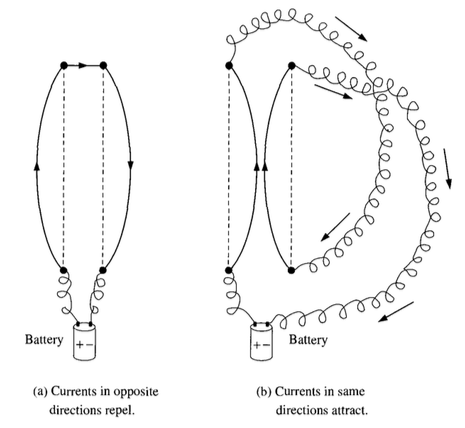
\includegraphics[width=0.98\textwidth]{./images/schematics/magnetic_force_between_wires_01.png}\\
    \end{center}
  \end{column}
  \begin{column}{0.40\textwidth}
   {\small
      As we saw in the previous lecture, there is a magnetic force exerted between two wires.\\
      This force is:
      \begin{itemize}
      {\small
         \item attractive if both currents flow in the same direction, and
         \item repulsive if the two currents flow in opposite directions.
      }
      \end{itemize}
   }
  \end{column}
\end{columns}

\end{frame}


%
%
%

\begin{frame}{Force between two parallel conductors}

\begin{columns}
  \begin{column}{0.40\textwidth}
    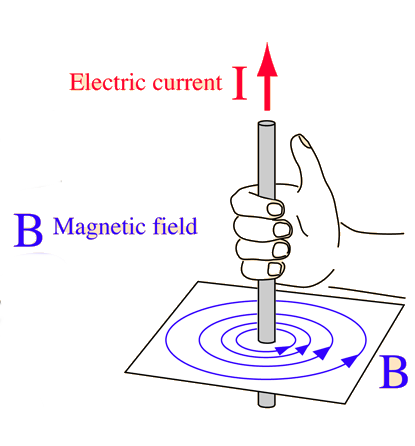
\includegraphics[width=0.85\textwidth]{./images/schematics/magnetic_field_around_wire_01.png}
  \end{column}
  \begin{column}{0.60\textwidth}
      We know the the magnetic field
      $\vec{B}$ produced by a constant current flowing across an infinite straight wire.
      \begin{equation*}
         \vec{B}(\vec{r})
             = \frac{\mu_0I}{2\pi \rho} \hat\phi
             = \frac{\mu_0I}{2\pi \rho} \Big( -\frac{y}{\rho}, \frac{x}{\rho}, 0 \Big)
     \end{equation*}
  \end{column}
\end{columns}

\vspace{0.2cm}

We also know the force exerted on a current within a magnetic field:
\begin{equation*}
  \vec{F} = I \int_{L} d\vec{\ell} \times \vec{B}
\end{equation*}

\vspace{0.1cm}

The two above ingredients allow us to
{\bf calculate the force between two parallel conductors.}\\

\end{frame}


%
%
%

\begin{frame}{Force between two parallel conductors}

Consider the 2 wires (1) and (2) shown below.\\
\vspace{0.2cm}

\begin{columns}
  \begin{column}{0.40\textwidth}
    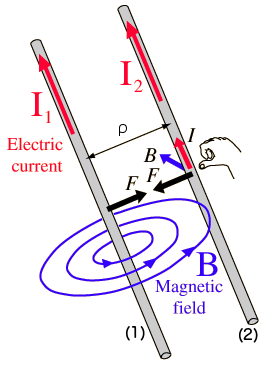
\includegraphics[width=0.90\textwidth]{./images/schematics/magnetic_force_between_wires_rho.png}\\
  \end{column}
  \begin{column}{0.60\textwidth}
     \begin{itemize}
       \item We will calculate the {\bf force $\vec{F}$ exerted on the current in wire (2)}.
       \item This force is {\bf caused by the magnetic field $\vec{B}$} at the location of wire (2)
                 {\bf due to the current in wire (1)}. (*)
     \end{itemize}
     \vspace{0.1cm}
     Convince yourselves, using the right-hand rule, that the magnetic force is:
     \begin{itemize}
         \item {\bf attractive} if both currents flow in the {\bf same direction}, and
         \item {\bf repulsive} if the two currents flow in {\bf opposite directions}.\\
     \end{itemize}
  \end{column}
\end{columns}
\vspace{0.1cm}
\noindent\rule{2cm}{0.4pt}\\
{\scriptsize
 (*)
     We will see that an {\bf interchange of (1) and (2) leaves the result unchanged}:
     i.e. the same result is obtained if we consider
     the force on wire (1) due to the field produced by wire (2).\\
}
\end{frame}

%
%
%

\begin{frame}{Force between two parallel conductors}

The force on wire (2) due to the field produced by wire (1) is:
\begin{equation*}
  \vec{F}_{21} = I_{2} \int d\vec{\ell}_{2} \times \vec{B}_{1}
\end{equation*}
where an infinitesimal element $d\vec{\ell}_{2}$ on wire (2) can be written as (*):
\begin{equation*}
  d\vec{\ell}_{2} = \Big( x, y, z+dz \Big) - \Big( x, y, z \Big) = \Big( 0, 0, dz \Big)
\end{equation*}
and the magnetic field due to wire (1) is:
\begin{equation*}
  \vec{B}_{1} = \frac{\mu_0I_{1}}{2\pi \rho} \Big( -\frac{y}{\rho}, \frac{x}{\rho}, 0 \Big)
\end{equation*}\\
\vspace{0.1cm}
Putting everything together,
the force $\vec{F}_{21}$ can be written as:
\begin{equation*}
  \vec{F}_{21} = \frac{\mu_0 I_{1} I_{2}}{2\pi \rho} \int \Big( 0, 0, dz \Big) \times \Big( -\frac{y}{\rho}, \frac{x}{\rho}, 0 \Big)
\end{equation*}

\noindent\rule{2cm}{0.4pt}\\
{\scriptsize
 (*) We take both wires to be along the z axis.
     Wire (1) passes through (x,y)=(0,0), whereas wire (2) passes through an arbitrary point on (x,y) plane.
}

\end{frame}

%
%
%

\begin{frame}{Force between two parallel conductors}

The cross product appearing in the previous equation can be calculated as:
\begin{equation*}
  \Big( 0, 0, dz \Big) \times \Big( -\frac{y}{\rho}, \frac{x}{\rho}, 0 \Big) =
   \left|
    \begin{array}{ccc}
      \hat{x}       & \hat{y}     & \hat{z} \\
       0            &  0          &  dz     \\
       -\frac{y}{\rho} & \frac{x}{\rho} &  0      \\
    \end{array}
   \right| =
\end{equation*}
\begin{equation*}
   \hat{x}
   \left|
    \begin{array}{cc}
       0          &  dz     \\
      \frac{x}{\rho} &  0      \\
    \end{array}
   \right| -
   \hat{y}
   \left|
    \begin{array}{cc}
       0            &  dz     \\
       -\frac{y}{\rho} &  0      \\
    \end{array}
   \right| +
   \hat{z}
   \left|
    \begin{array}{cc}
       0            &  0          \\
       -\frac{y}{\rho} & \frac{x}{\rho} \\
    \end{array}
   \right| =
  \Big( -\frac{x}{\rho}, -\frac{y}{\rho}, 0 \Big) dz
\end{equation*}

\vspace{0.1cm}

Therefore:
\begin{equation*}
  \vec{F}_{21} =
     \frac{\mu_0 I_{1} I_{2}}{2\pi \rho} \int_{L} \Big( -\frac{x}{\rho}, -\frac{y}{\rho}, 0 \Big) dz =
     - \frac{\mu_0 I_{1} I_{2}}{2\pi \rho} \int_{L} \Big(\frac{x}{\rho}, \frac{y}{\rho}, 0 \Big) dz
\end{equation*}

The vector $\Big(\frac{x}{\rho}, \frac{y}{\rho}, 0 \Big)$ is a
constant for the integration over the length L of the wire, hence:
\begin{equation*}
  \vec{F}_{21} =
       - \frac{\mu_0 I_{1} I_{2}}{2\pi \rho} \Big(\frac{x}{\rho}, \frac{y}{\rho}, 0 \Big) \int_{L} dz
\end{equation*}

\end{frame}

%
%
%


\begin{frame}{Force between two parallel conductors}

Performing the trivial integration over z, we have:
\begin{equation*}
  \vec{F}_{21} = - \frac{\mu_0 I_{1} I_{2} L}{2\pi \rho} \Big(\frac{x}{\rho}, \frac{y}{\rho}, 0 \Big)
\end{equation*}

\vspace{0.2cm}

\begin{columns}
  \begin{column}{0.16\textwidth}
   \begin{center}
    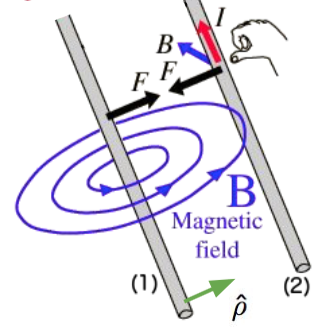
\includegraphics[width=0.90\textwidth]{./images/schematics/magnetic_force_between_wires_rho_hat.png}\\
   \end{center}
  \end{column}
  \begin{column}{0.84\textwidth}
   {\small
     What is $\Big(\frac{x}{\rho}, \frac{y}{\rho}, 0 \Big)$?
    It can be easily seen that it is the unit vector $\hat{\rho}$, pointing along the (shortest) distance between wires (1) and (2).
    \begin{equation*}
      \hat{\rho} = \Big(\frac{x}{\rho}, \frac{y}{\rho}, 0 \Big) \; , \;
      \hat{\rho} \cdot \hat{\rho} = \Big( \frac{x}{\rho} \Big)^2 +  \Big( \frac{y}{\rho} \Big)^2 = 1
    \end{equation*}
   }
  \end{column}
\end{columns}

\vspace{0.2cm}

The force $\vec{F}_{21}$ on wire (2) due to the field of wire (1) is written as:
\begin{equation*}
  \vec{F}_{21} = - \frac{\mu_0 I_{1} I_{2} L}{2\pi \rho} \hat{\rho}
\end{equation*}

\end{frame}

%
%
%

\begin{frame}{Force between two parallel conductors}

The force $\vec{F}_{21}$ on wire (2) due to the field of wire (1):
\begin{equation*}
  \vec{F}_{21} = - \frac{\mu_0 I_{1} I_{2} L}{2\pi \rho} \hat{\rho}
\end{equation*}

\begin{columns}
  \begin{column}{0.70\textwidth}
    \begin{center}
      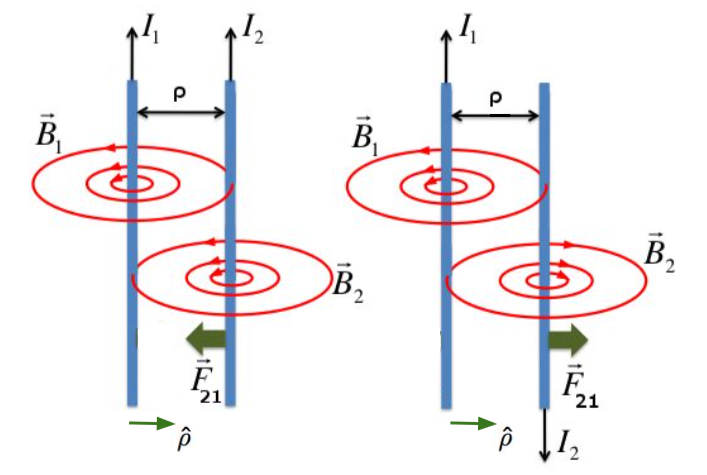
\includegraphics[width=0.98\textwidth]{./images/schematics/magnetic_force_between_wires_2_cases_02.png}\\
    \end{center}
  \end{column}
  \begin{column}{0.30\textwidth}
     The presence of $-\hat{\rho}$ tells us that, if $I_1$ and $I_2$ have the same direction,
     the force  $\vec{F}_{21}$ pulls the wire (2) towards the wire (1).
  \end{column}
\end{columns}

\end{frame}

%
%
%

\begin{frame}{Force between two parallel conductors}

Consequently, the force $\vec{F}_{12}$ on wire (1) due to the field of wire (2) is given by:
\begin{equation*}
  \vec{F}_{12} = - \frac{\mu_0 I_{1} I_{2} L}{2\pi \rho} \hat{\rho^{\prime}} = \frac{\mu_0 I_{1} I_{2} L}{2\pi \rho} \hat{\rho}
\end{equation*}

\begin{columns}
  \begin{column}{0.70\textwidth}
    \begin{center}
      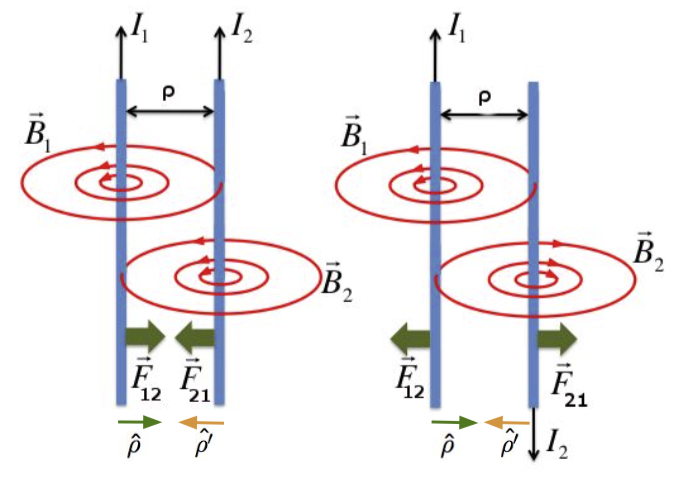
\includegraphics[width=0.98\textwidth]{./images/schematics/magnetic_force_between_wires_2_cases_03.png}\\
    \end{center}
  \end{column}
  \begin{column}{0.30\textwidth}
     The relative minus sign is because the corresponding unit vector $\hat{\rho^{\prime}}$ starting
     from wire (2) and pointing towards wire (1) has the opposite direction wrt $\hat{\rho}$:
     $\hat{\rho^{\prime}}$ = -$\hat{\rho}$
  \end{column}
\end{columns}

\end{frame}


%
%
%

\begin{frame}{Force between two parallel conductors}

The force $\vec{F}_{21}$ on wire (2) due to the field of wire (1):
\begin{equation*}
  \vec{F}_{21} = - \frac{\mu_0 I_{1} I_{2} L}{2\pi \rho} \hat{\rho}
\end{equation*}

The force $\vec{F}_{12}$ on wire (1) due to the field of wire (2):
\begin{equation*}
  \vec{F}_{12} = - \frac{\mu_0 I_{1} I_{2} L}{2\pi \rho} \hat{\rho^{\prime}} = \frac{\mu_0 I_{1} I_{2} L}{2\pi \rho} \hat{\rho}
\end{equation*}

Notice that in both cases, the magnitude of the force is the same, as expected:
\begin{equation*}
  |\vec{F}_{21}| =  |\vec{F}_{12}| = \frac{\mu_0 I_{1} I_{2} L}{2\pi \rho}
\end{equation*}

From now on we will drop the indices from the force and write it as:
\begin{equation*}
  F = \frac{\mu_0 I_{1} I_{2} L}{2\pi \rho}
\end{equation*}

\end{frame}


%
% Worked example
%

{
\setbeamercolor {frametitle} {bg=eBG1}
\setbeamercolor {author in head/foot} {bg=eBG1}
\setbeamercolor {title in head/foot} {bg=eBG2}
\setbeamercolor {date in head/foot} {bg=eBG3}
\setbeamercolor {date in head/foot} {fg=eFG3}

%
%
%

\begin{frame}{Worked example}

\begin{blockexmplque}{Question}

\begin{columns}
  \begin{column}{0.30\textwidth}
    \begin{center}
      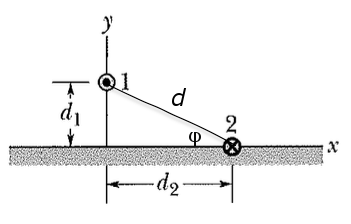
\includegraphics[width=0.98\textwidth]{./images/problems/lect5_force_2wires.png}\\
    \end{center}
  \end{column}
  \begin{column}{0.70\textwidth}
    {\small
        The figure on the left shows wire 1 in cross section; the wire
        is long and straight, carries a current of 4.00 mA out of the
        page, and is at distance $d_1$ = 2.40 cm from a surface.
        Wire 2, which is parallel to wire 1 and also long,  is at
        horizontal distance $d_2$ = 5.00 cm from wire 1 and carries a
        current of 6.80 mA into the page.\\
    }
  \end{column}
\end{columns}
\vspace{0.2cm}
What is the x-component of
the magnetic force {\em per unit length} on wire 2 due to wire 1?
\end{blockexmplque}

\vspace{0.3cm}

{\small
 The magnitude of the force per unit length between the wires is given by:
\begin{equation*}
  \frac{F}{L} = \frac{\mu_0 I_{1} I_{2}}{2\pi d} \Rightarrow
  \frac{F}{L} = \frac{\mu_0 I_{1} I_{2}}{2\pi \sqrt{d_1^2+d_2^2}}
\end{equation*}
}
\end{frame}

%
%
%

\begin{frame}{Worked example}

\begin{columns}
  \begin{column}{0.30\textwidth}
    \begin{center}
      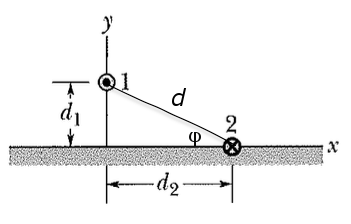
\includegraphics[width=0.98\textwidth]{./images/problems/lect5_force_2wires.png}\\
    \end{center}
  \end{column}
  \begin{column}{0.70\textwidth}
   {\small
     The x-component is found by multiplying the amplitude with:
     \begin{equation*}
        cos\phi =  \frac{d_2}{\sqrt{d_1^2+d_2^2}}
     \end{equation*}
   }
  \end{column}
\end{columns}


{\small

Therefore, the x-component of
the magnetic force {\em per unit length} on wire 2 due to wire 1 is:

\begin{equation*}
 \frac{F_x}{L} =
     \frac{\mu_0 I_{1} I_{2}}{2\pi \sqrt{d_1^2+d_2^2}} \cdot
     \frac{d_2}{\sqrt{d_1^2+d_2^2}} \Rightarrow
 \frac{F_x}{L} =
      \frac{\mu_0 I_{1} I_{2} d_2}{2\pi (d_1^2+d_2^2)} \Rightarrow
\end{equation*}

\begin{equation*}
 \frac{F_x}{L} =
    \frac{ (4\pi \times 10^{-7} \; T \cdot m/A)
              (4.00 \times 10^{-3}\; A)
              (6.80 \times 10^{-3}\; A)
              (0.050 \; m)}
          {2\pi \Big( (0.024\; m)^2+(0.050\; m)^2 \Big)} \Rightarrow
\end{equation*}

\begin{equation*}
 \frac{F_x}{L} = 8.84 \times 10^{-11} \; N/m
\end{equation*}

}
\end{frame}

} % worked example


%
%
%

\begin{frame}{The definition of an Ampere}

The force between two conducting wires
\begin{equation*}
   F = \frac{\mu_0 I_{1} I_{2} L}{2\pi \rho}
\end{equation*}

is used to {\bf define the SI unit of current (Ampere)}\\

\vspace{0.3cm}

Assume:
\begin{itemize}
  \item 2 straight parallel conductors, placed in vacuum
  \item The conductors are 1 m apart
  \item They have infinite length and negligible cross section.\\
\end{itemize}

\vspace{0.3cm}

One {\bf Ampere is the amount of current that},
if maintained between those conductors {\bf produces a force of 2 $\times$ $10^{-7}$ N per metre of length.}

\end{frame}

%
%
%

\begin{frame}{Current loop}

\begin{columns}
  \begin{column}{0.40\textwidth}
    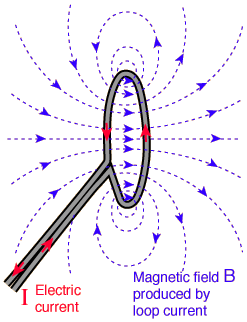
\includegraphics[width=0.99\textwidth]{./images/schematics/current_loop.png}\\
  \end{column}
  \begin{column}{0.60\textwidth}
        Let's consider a {\bf current loop} as the one shown on the left.\\
        \vspace{0.3cm}
        {\small
        A current loop is a {\bf magnetic dipole} which is the magnetic analogue of the
        electric dipole we saw at an earlier lecture. The analogies
        will become clearer later in this lecture series.\\
        }
  \end{column}
\end{columns}

\end{frame}

%
%
%

\begin{frame}{A current loop within a magnetic field}

Let's study a {\bf conducting loop within a magnetic field}.\\
\vspace{0.3cm}
\begin{columns}
  \begin{column}{0.30\textwidth}
    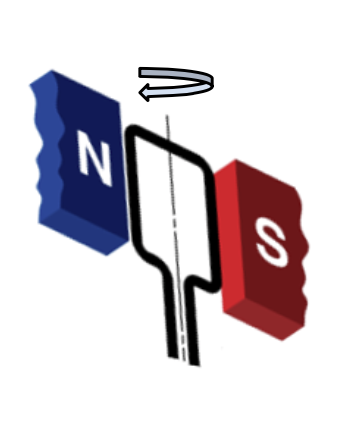
\includegraphics[width=0.99\textwidth]{./images/schematics/current_loop_in_magnetic_field.png}\\
  \end{column}
  \begin{column}{0.70\textwidth}
     {\small
      For simplicity, we will examine:
      \begin{itemize}
      {\small
        \item a loop with a {\bf rectangular shape},
        \item circulated by a {\bf constant current I},
        \item placed within a {\bf uniform magnetic field B} that is {\bf perpendicular to the long sides}.
      }
      \end{itemize}
     }
  \end{column}
\end{columns}
We will assume that the loop can {\bf rotate freely around an axis} parallel
to the long sides going through the centre of the short sides (see figure).\\

\end{frame}

%
%
%

\begin{frame}{Force on the sides of a current loop}

\begin{columns}
  \begin{column}{0.37\textwidth}
    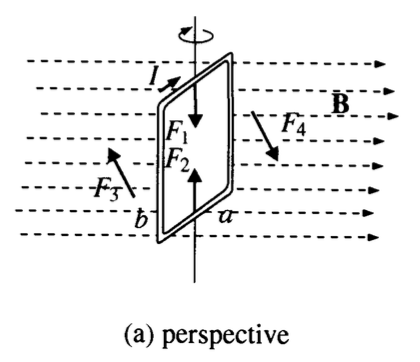
\includegraphics[width=0.99\textwidth]{./images/schematics/magnetic_torque_current_loop_perspective.png}\\
    \vspace{0.3cm}
    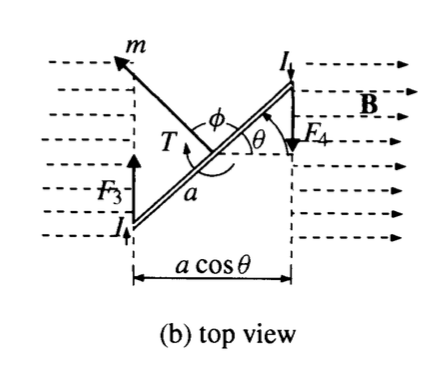
\includegraphics[width=0.99\textwidth]{./images/schematics/magnetic_torque_current_loop_top_view.png}\\
  \end{column}
  \begin{column}{0.63\textwidth}
  {\small
    We will study the force exerted on each side of the loop.
    This force, as we have seen, is given by:
    \begin{equation*}
        \vec{F} = I \int_{L} d\vec{\ell} \times \vec{B}
    \end{equation*}
    \vspace{0.1cm}
    Its direction is given by the right-hand rule.\\
    \begin{center}
      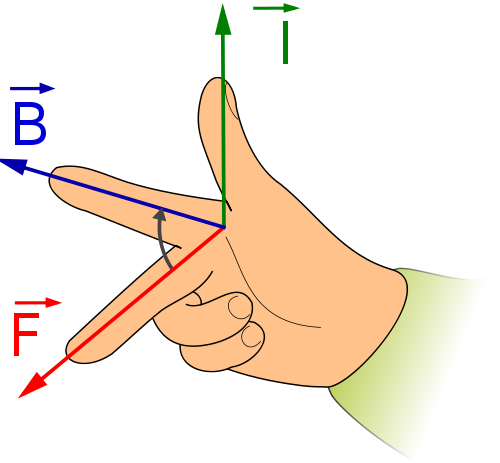
\includegraphics[width=0.30\textwidth]{./images/schematics/right_hand_rule_fbi.png}\\
    \end{center}
    Let {\bf a} be the length of the short sides, and {\bf b} the length of the long sides.
    As the loop rotates, the angle between the short sides and the magnetic field $\vec{B}$ changes:
    Let's call this angle $\theta$ (see figure).\\
  }
  \end{column}
\end{columns}

\end{frame}


%
%
%

\begin{frame}{Force on the sides of a current loop}

\begin{columns}
  \begin{column}{0.37\textwidth}
    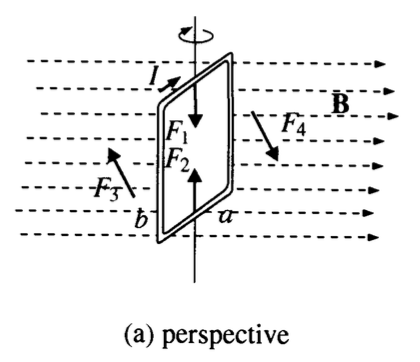
\includegraphics[width=0.99\textwidth]{./images/schematics/magnetic_torque_current_loop_perspective.png}\\
    \vspace{0.3cm}
    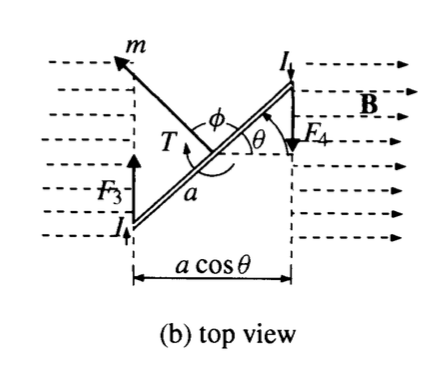
\includegraphics[width=0.99\textwidth]{./images/schematics/magnetic_torque_current_loop_top_view.png}\\
  \end{column}
  \begin{column}{0.63\textwidth}
  {\small
    $|\vec{B}|$ is constant over the loop,
    but, as it (the loop) rotates, the angle between the short sides (and, hence, their current)
    and $\vec{B}$ changes.\\
    \vspace{0.2cm}
    Therefore, the force on the short sides is:
    \begin{equation*}
      |\vec{F}_1| = |\vec{F}_2| = I a |\vec{B}| sin\theta
    \end{equation*}
    where the angle $\theta$ was defined previously.
    Obviously, as the loop rotates the force on the short sides varies between:
    \begin{equation*}
      |\vec{F}_1| = |\vec{F}_2| =
        \left\{
          \begin{array}{l}
             0, \text{for $\theta = 0$, and} \\
             I a |\vec{B}|, \text{for $\theta = \pi/2$}
          \end{array}
        \right.
    \end{equation*}
    On the other hand, the long sides are perpendicular to $\vec{B}$
    and, hence, the force on them is constant and is given by:
    \begin{equation*}
      |\vec{F}_3| = |\vec{F}_4| = I b |\vec{B}|
    \end{equation*}
  }
  \end{column}
\end{columns}

\end{frame}

%
%
%

\begin{frame}{Direction of forces on the sides of a current loop}

\begin{columns}
  \begin{column}{0.37\textwidth}
    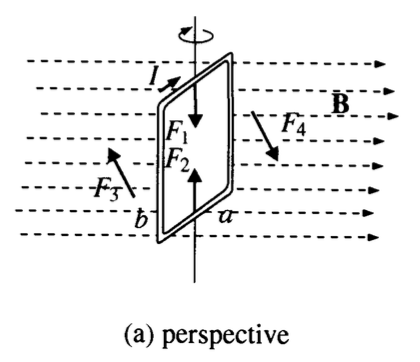
\includegraphics[width=0.99\textwidth]{./images/schematics/magnetic_torque_current_loop_perspective.png}\\
    \vspace{0.3cm}
    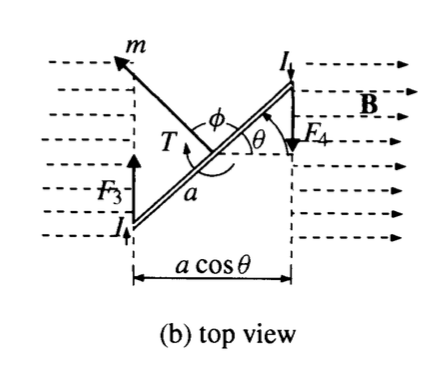
\includegraphics[width=0.99\textwidth]{./images/schematics/magnetic_torque_current_loop_top_view.png}\\
  \end{column}
  \begin{column}{0.63\textwidth}
  {\small
    Using the right-hand rule, one can easily see that the forces on the
    short sides ($\vec{F}_1$ and $\vec{F}_2$) are either:
    \begin{itemize}
        \item both pointing inwards trying to {\em squeeze} the loop (for $ 0 < \theta < \pi$), or
        \item both pointing outwards trying to {\em expand} the loop (for $\pi < \theta < 2\pi$).
    \end{itemize}
    On either case, the forces on the short sides are parallel to the axis or rotation,
    hence they exert {\bf no torque on the loop}.\\
    \vspace{0.2cm}
    On the other hand, the forces on the two long sides ($\vec{F}_3$ and $\vec{F}_4$)
    have constant but opposite directions. They are perpendicular to the axis of rotation and,
    therefore, {\bf they exert a torque on the loop}.\\
  }
  \end{column}
\end{columns}

\end{frame}


%
%
%

\begin{frame}{Torque on a current loop}

\begin{columns}
  \begin{column}{0.37\textwidth}
    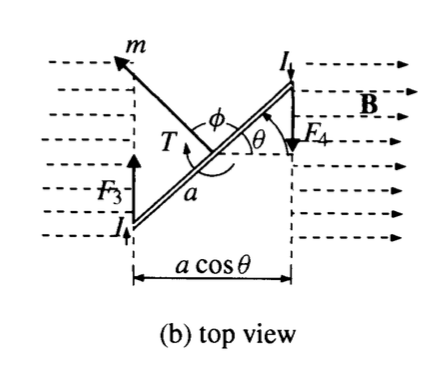
\includegraphics[width=0.99\textwidth]{./images/schematics/magnetic_torque_current_loop_top_view.png}\\
  \end{column}
  \begin{column}{0.63\textwidth}
  {\small
     The torque $\vec{T}$ exerted by a force $\vec{F}$ is:
     \begin{equation*}
         \vec{T} = \vec{r} \times \vec{F}
     \end{equation*}
      where $\vec{r}$ is the displacement vector,
      pointing from the axis of rotation to the point where the force is applied.
  }
  \end{column}
\end{columns}
In our case (see figure above) $\vec{T}$ (which points into the page, $\hat{in}$) is:
\begin{equation*}
     \vec{T} =
        \bigg\{ \frac{a}{2} |F_{3}| sin \Big(\frac{\pi}{2}+\theta \Big) +
                \frac{a}{2} |F_{4}| sin \Big(\frac{\pi}{2}+\theta \Big) \bigg\} \hat{in}
        \xRightarrow {|F_{3}| = |F_{4}| =  I b |\vec{B}|}
\end{equation*}
\begin{equation*}
      \vec{T} =
         \cancel{2} \frac{a}{\cancel{2}}
            \Big( I b |\vec{B}| \Big) sin\Big(\frac{\pi}{2}+\theta \Big) \hat{in} =
         I \Big( a \; b \Big) |\vec{B}| sin\Big(\frac{\pi}{2}+\theta \Big) \hat{in}
        \xRightarrow {|\vec{S}| = ab,\;\; \phi = \frac{\pi}{2}+\theta = \angle(\vec{S},\vec{B})}
\end{equation*}
\begin{equation*}
      \vec{T} = \Big( I \vec{S} \Big) \times \vec{B}
\end{equation*}

\end{frame}

%
%
%

\begin{frame}{Magnetic dipole moment}

The {\bf magnetic dipole moment} $\vec{m}$ of a current loop is defined as
\begin{equation*}
  \vec{m} = I \vec{S}
\end{equation*}

The magnetic moment of a magnet is a quantity that
{\bf determines the torque it will experience in an external magnetic field.}

\begin{columns}
  \begin{column}{0.30\textwidth}
    \begin{center}
      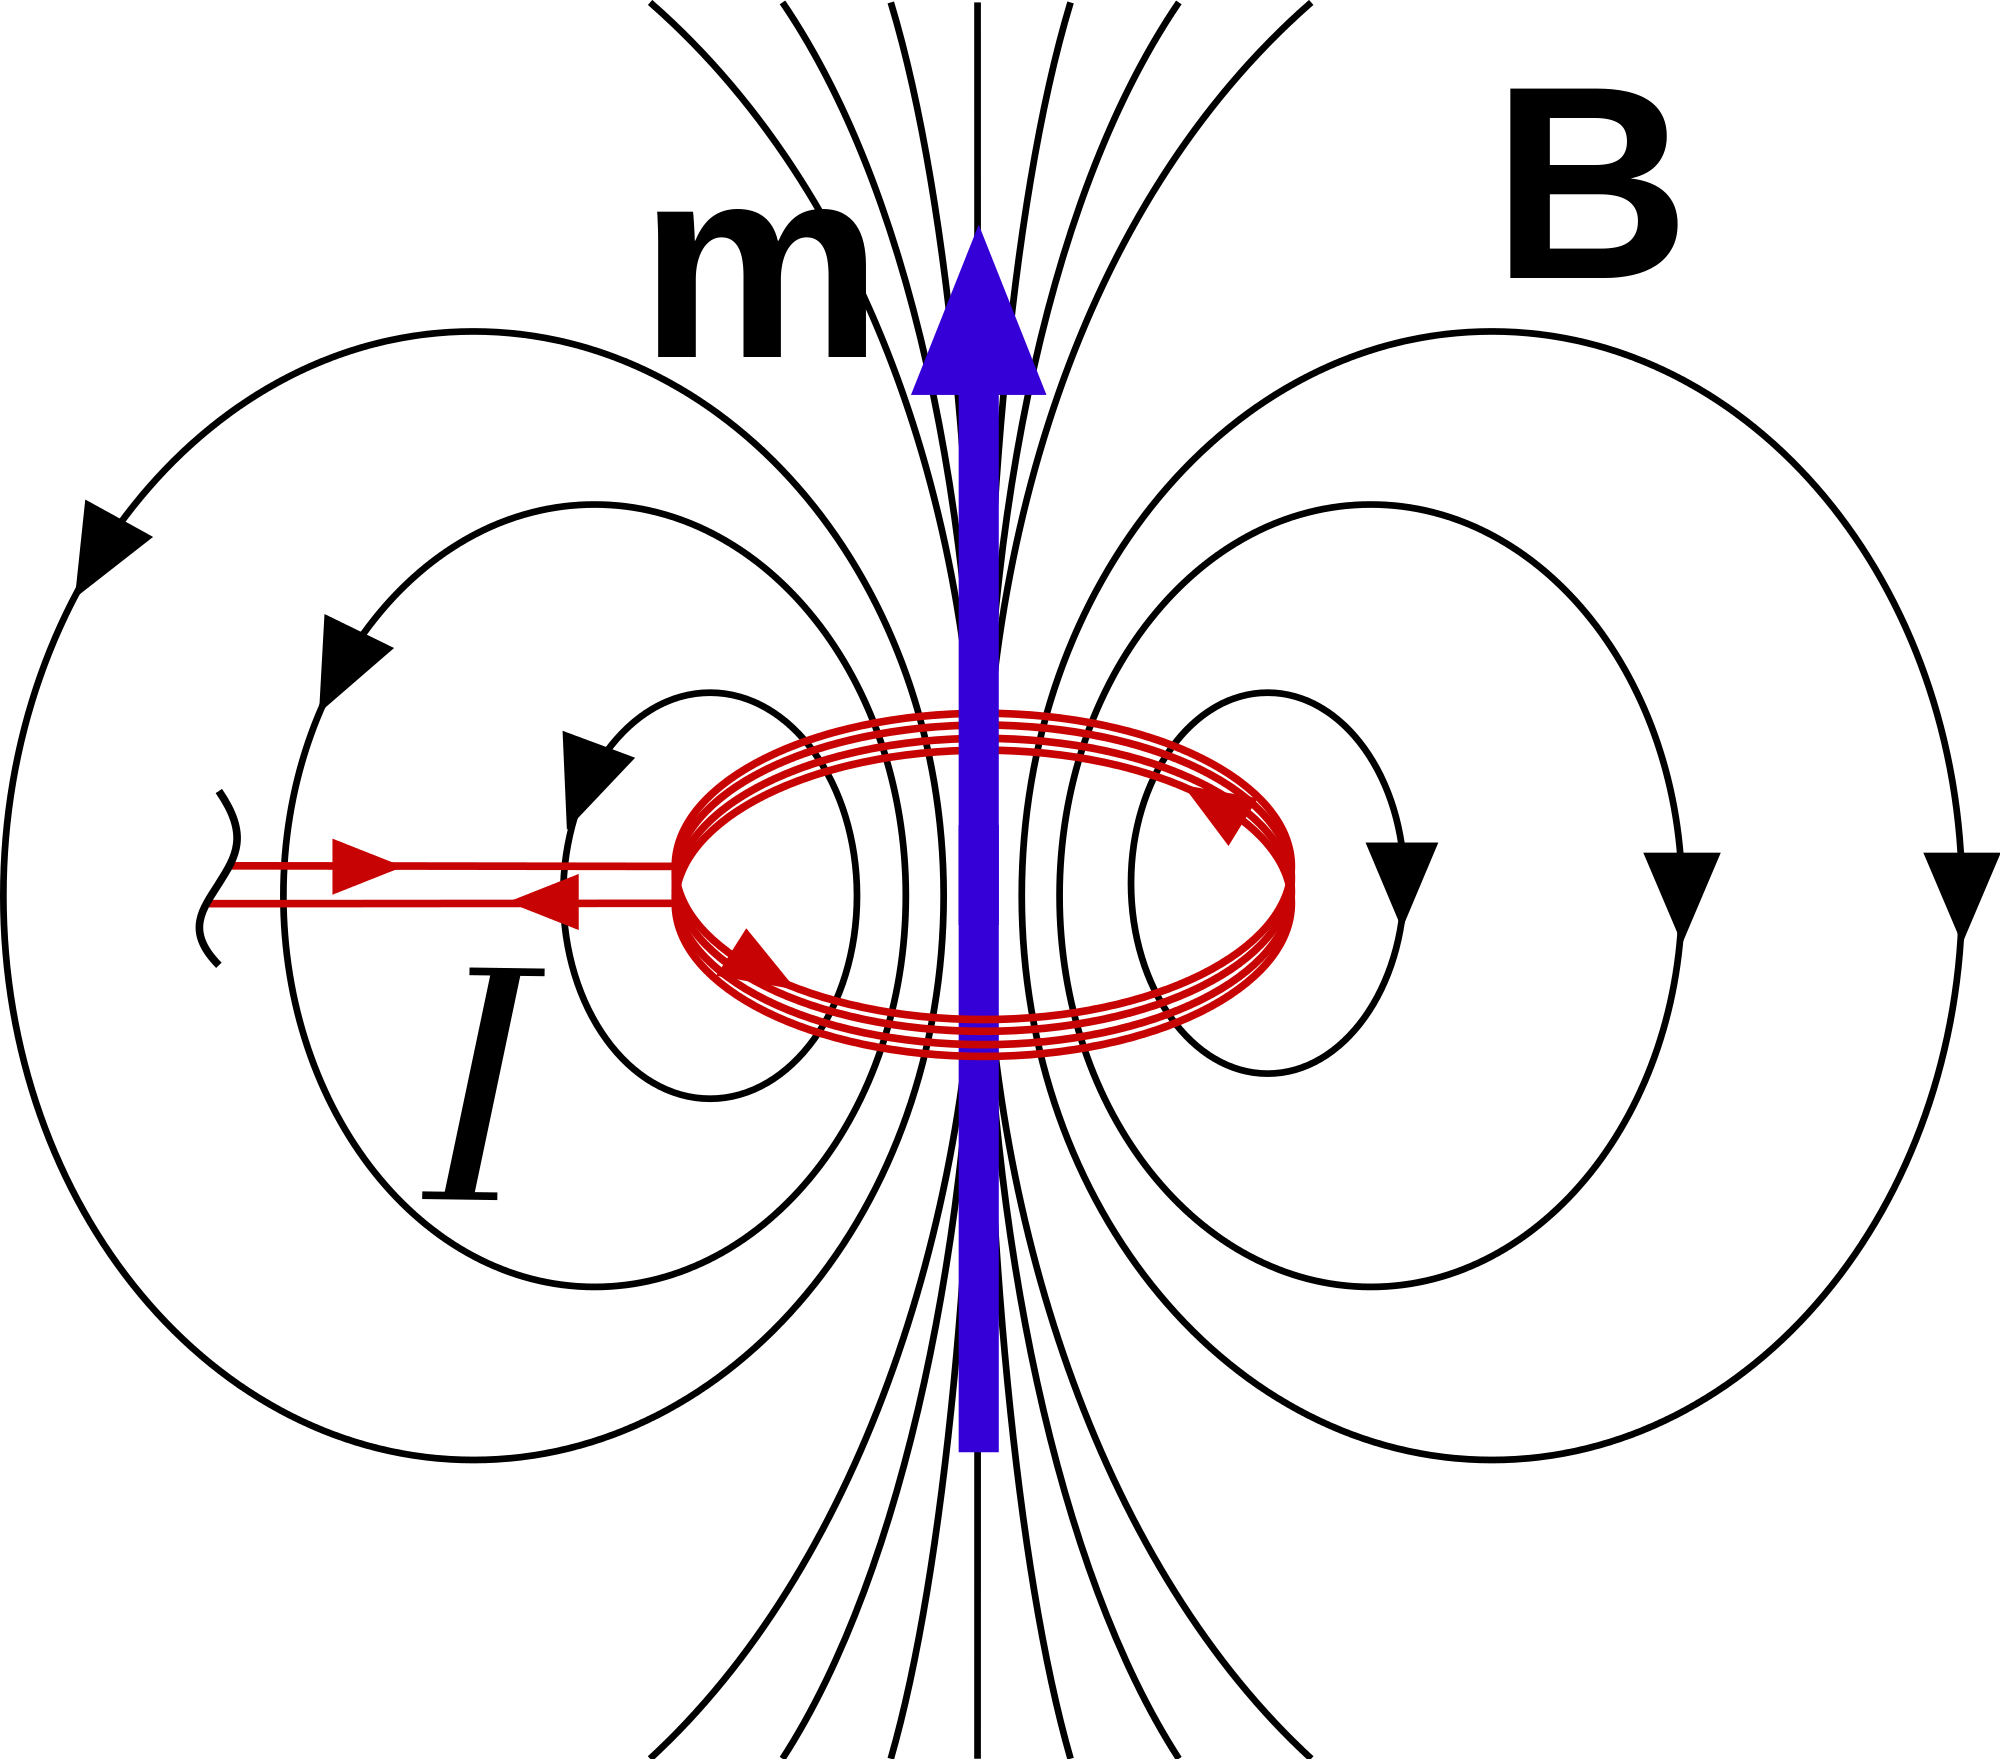
\includegraphics[width=0.75\textwidth]{./images/schematics/magnetic_dipole_moment_02.png}
      \vspace{0.2cm}
      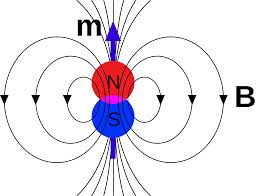
\includegraphics[width=0.75\textwidth]{./images/schematics/magnetic_dipole_moment_01.jpg}\\
    \end{center}
  \end{column}
  \begin{column}{0.70\textwidth}
  {\small
     The magnetic dipole moment is {\bf a vector}.
     it has both a magnitude ($|\vec{m}|$ = I $|\vec{S}|$) and a direction:
     \begin{itemize}
       \item Curl your right hand in the direction of the current in the loop: Your thumb points towards the magnetic dipole moment.
       \item You can also think that it points from the south to north pole of the magnet.
     \end{itemize}
   }
  \end{column}
\end{columns}

\end{frame}


%
%
%

\begin{frame}{Magnetic dipole moment for any planar loop}

Is the simple definition of the magnetic dipole moment $\vec{m}$
\begin{equation*}
  \vec{m} = I \vec{S}
\end{equation*}
a consequence of considering a simple loop with a rectangular shape?\\

\begin{columns}
  \begin{column}{0.40\textwidth}
     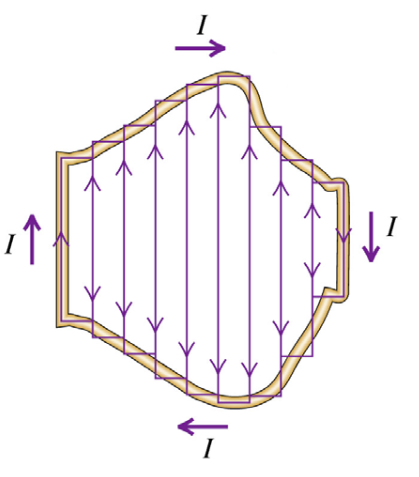
\includegraphics[width=0.98\textwidth]{./images/schematics/current_loop_irregular_shape.png}\\
  \end{column}
  \begin{column}{0.60\textwidth}
      {\bf What if the current loop had an arbitrary shape?}\\
     \vspace{0.3cm}
      Any planar current loop of any shape can be approximated by a
      set of rectangular loops.
  \end{column}
\end{columns}

\end{frame}

%
% Worked example
%

{
\setbeamercolor {frametitle} {bg=eBG1}
\setbeamercolor {author in head/foot} {bg=eBG1}
\setbeamercolor {title in head/foot} {bg=eBG2}
\setbeamercolor {date in head/foot} {bg=eBG3}
\setbeamercolor {date in head/foot} {fg=eFG3}

%
%
%

\begin{frame}{Worked example}

\begin{blockexmplque}{Question}

\begin{columns}
  \begin{column}{0.30\textwidth}
    \begin{center}
      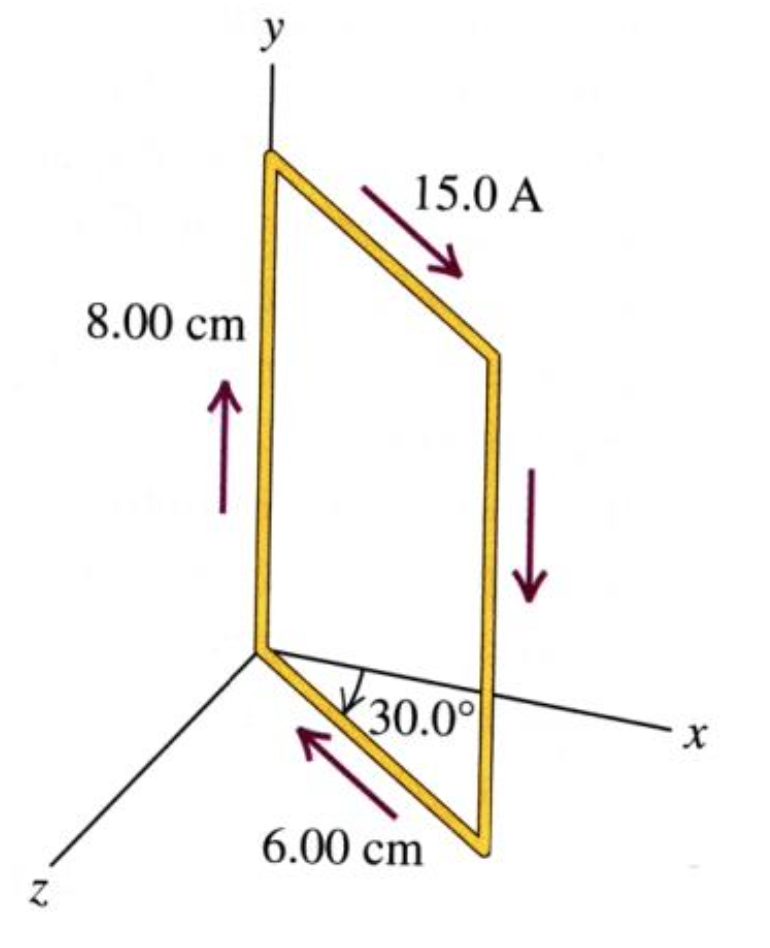
\includegraphics[width=0.98\textwidth]{./images/problems/lect5_rectangular_loop}\\
    \end{center}
  \end{column}
  \begin{column}{0.70\textwidth}
    {\small
       The rectangular loop in the figure is pivoted around the y-axis and
       carries a current of 15.0 A in the direction shown.
       \begin{enumerate}
       {\small
          \item
             If the loop is in uniform magnetic field with magnitude 0.48 T in the +x direction,
             find the magnitude and direction of the torque required to hold the loop
             in the position shown.
         \item
             What torque would be required if the loop were pivoted about an axis
            through its centre, parallel to the y-axis?
       }
       \end{enumerate}
   }
  \end{column}
\end{columns}
\end{blockexmplque}

\vspace{0.3cm}

{\small
        (1) The torque exerted by a field $\vec{B}$ on a magnetic dipole moment $\vec{m}$ is:
         \begin{equation*}
            \vec{T} = \vec{m} \times \vec{B}
         \end{equation*}
}

\end{frame}


%
%
%

\begin{frame}{Worked example}

\begin{columns}[T]
  \begin{column}{0.30\textwidth}
    \begin{center}
      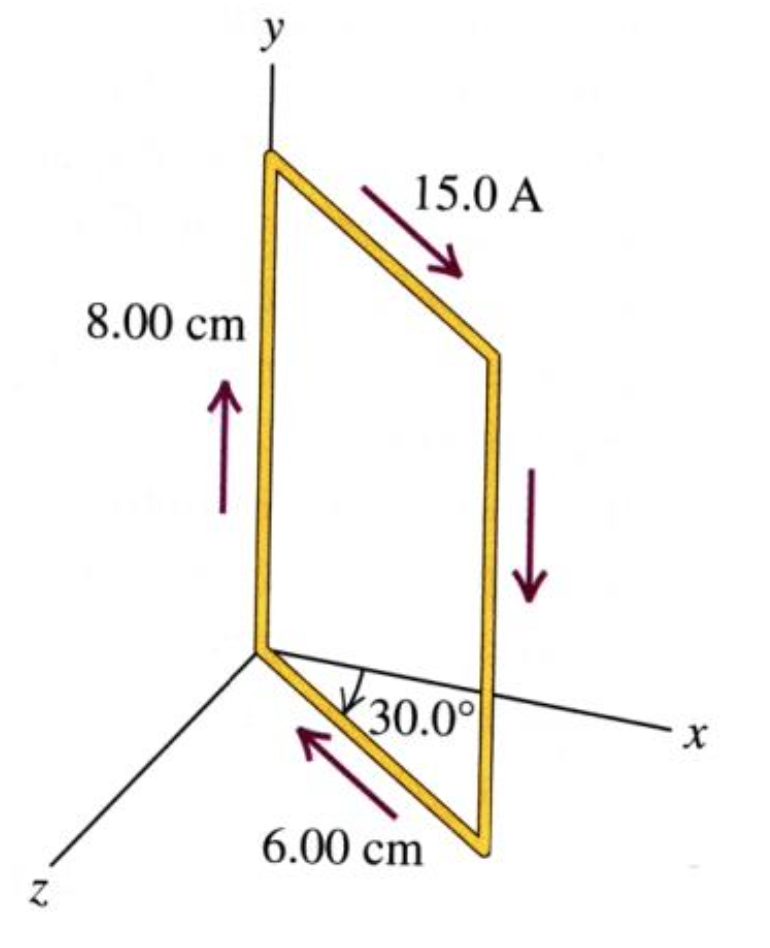
\includegraphics[width=0.98\textwidth]{./images/problems/lect5_rectangular_loop}\\
    \end{center}
  \end{column}
  \begin{column}{0.70\textwidth}
   {\small
         $\vec{B}$ is along $\hat{x}$ and $\vec{m}$ is perpendicular to the loop and towards the direction of
         your thumb if your right-hand curls in the direction of the
         current. \\
         \vspace{0.2cm}
         In the position shown, $\vec{m}$
         is on the xz plane pointing towards
         $\hat{n}$ = - cos$\displaystyle \frac{\pi}{6}$ $\hat{z}$ + sin$\displaystyle \frac{\pi}{6}$ $\hat{x}$.\\
         \vspace{0.2cm}
         Therefore, the direction of the torque exerted by the
         magnetic field is towards the negative y axis ($-\hat{y}$):\\
         To keep the loop in place,
         you must provide a torque in the opposite direction  ($+\hat{y}$).\\
   }
  \end{column}
\end{columns}

{\small
         The magnitude of $\vec{T}$  is:
         \begin{equation*}
            |\vec{T}| = |\vec{m}| \cdot |\vec{B}| \cdot  sin\Big( \angle(\vec{m},\vec{B}) \Big) \Rightarrow
            |\vec{T}| = \Big( I \cdot S \Big) \cdot |\vec{B}| \cdot  sin\Big( \angle(\vec{m},\vec{B}) \Big) \Rightarrow
         \end{equation*}
         \begin{equation*}
            |\vec{T}| = \Big( 15.0 \; A \cdot 0.08 \; m  \cdot 0.06 \; m \Big) \cdot \Big( 0.48 \; T \Big)
               \cdot  sin \Big( \frac{\pi}{2} - \frac{\pi}{6} \Big) \Rightarrow
         \end{equation*}
}

\end{frame}

%
%
%

\begin{frame}{Worked example}

\begin{columns}[T]
  \begin{column}{0.30\textwidth}
    \begin{center}
      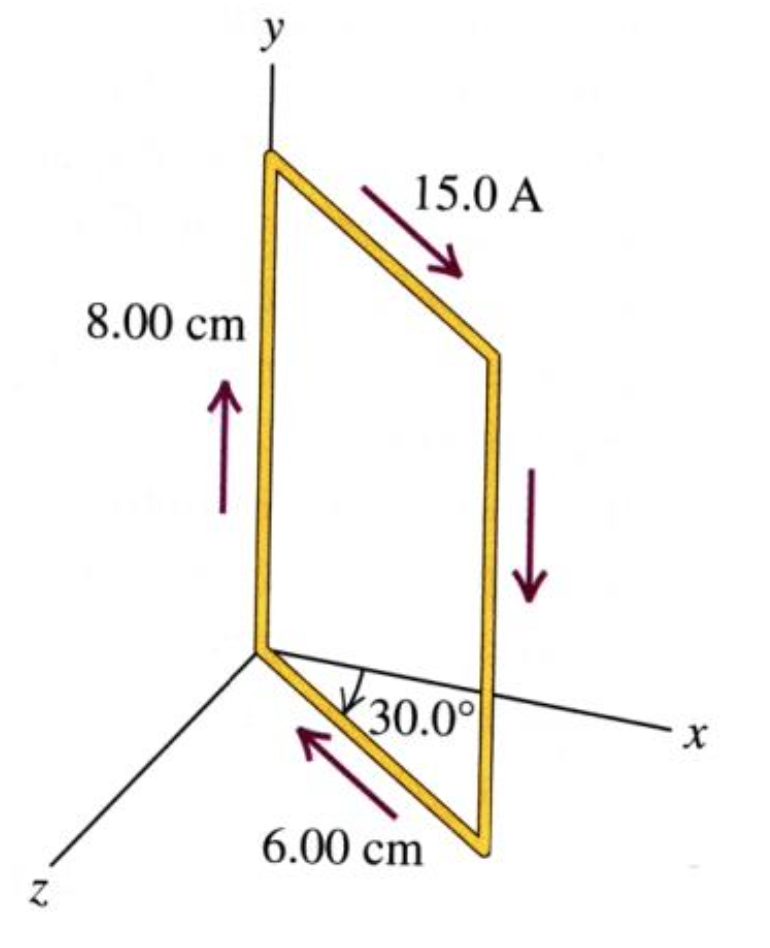
\includegraphics[width=0.98\textwidth]{./images/problems/lect5_rectangular_loop}\\
    \end{center}
  \end{column}
  \begin{column}{0.70\textwidth}
  {\small
         \begin{equation*}
            |\vec{T}| = \Big( 15.0 \cdot 0.08 \cdot 0.06 \cdot 0.48 \; sin \frac{\pi}{3} \Big) \; N \cdot m \Rightarrow
         \end{equation*}
         \begin{equation*}
            |\vec{T}| \approx 0.03 \; N \cdot m
         \end{equation*}
         \vspace{0.3cm}

          (2) If the loop was pivoted through its center, then there would be a torque on
          both sides of the loop parallel to the rotation axis. However, the lever arm
          is only half as large, so the total torque in each case is identical to the value found in part (1).
   }
  \end{column}
\end{columns}


\end{frame}


} % Worked example

%
%
%

\begin{frame}{The electric motor}

As we have seen:
\begin{itemize}
  \item an electric currents induces a magnetic field, and
  \item a moving magnet (or an otherwise varying magnetic field) induces an electric current
\end{itemize}

And, as we also saw earlier today:
\begin{itemize}
   \item A magnetic field exerts a torque on a current loop and spins it!
\end{itemize}

\vspace{0.2cm}

The exciting question, very early on, was:
{\bf Could we exploit these phenomena to build engines to do work?}
\begin{itemize}
  \item The relevant empirical laws were already known by the early 1820's.
  \item Already at the end of that decade there were early versions of {\em \bf electrical motors.}
\end{itemize}

\noindent\rule{2cm}{0.4pt}\\
{\scriptsize
Read {\em `The invention of the electric motor 1800-1854' }
by Martin Doppelbauer,
available at: https://www.eti.kit.edu/english/1376.php\\
}

\end{frame}

%
%
%

\begin{frame}{The electric motor}

\begin{columns}
  \begin{column}{0.40\textwidth}
   {\scriptsize
     \begin{center}
           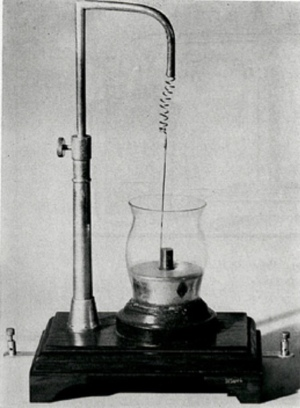
\includegraphics[width=0.90\textwidth]{./images/photos/rotating_wire_faraday.jpg}\\
            Michael Faraday, 1821:
            A vertically suspended wire moves in a circular orbit around a magnet.
     \end{center}
   }
  \end{column}
  \begin{column}{0.60\textwidth}
     \begin{center}
   {\scriptsize
     \begin{center}
           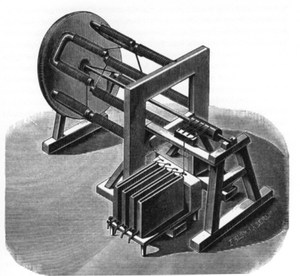
\includegraphics[width=0.45\textwidth]{./images/photos/electric_motor_jacobi_1834.jpg}\\
            Moritz Jacobi, 1834:
            First (?) electric motor (15 W)\\
            \vspace{0.2cm}
            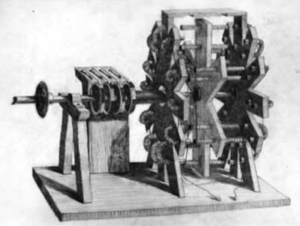
\includegraphics[width=0.45\textwidth]{./images/photos/electric_motor_improved_jacobi_1838.jpg}\\
            Moritz Jacobi, 1838:
            Improved electric motors (300 W, 1/4 hp) - Could propel a boat with a dozen passengers on a 7.5 km
            journey at a speed of 2.5 km/h.\\
     \end{center}
   }
     \end{center}
  \end{column}
\end{columns}


\end{frame}


%
%
%

\begin{frame}{The electric motor}

{\bf An electric motor is a machine that converts electrical energy into mechanical energy.}

\begin{columns}
  \begin{column}{0.50\textwidth}
   {\scriptsize
     \begin{center}
           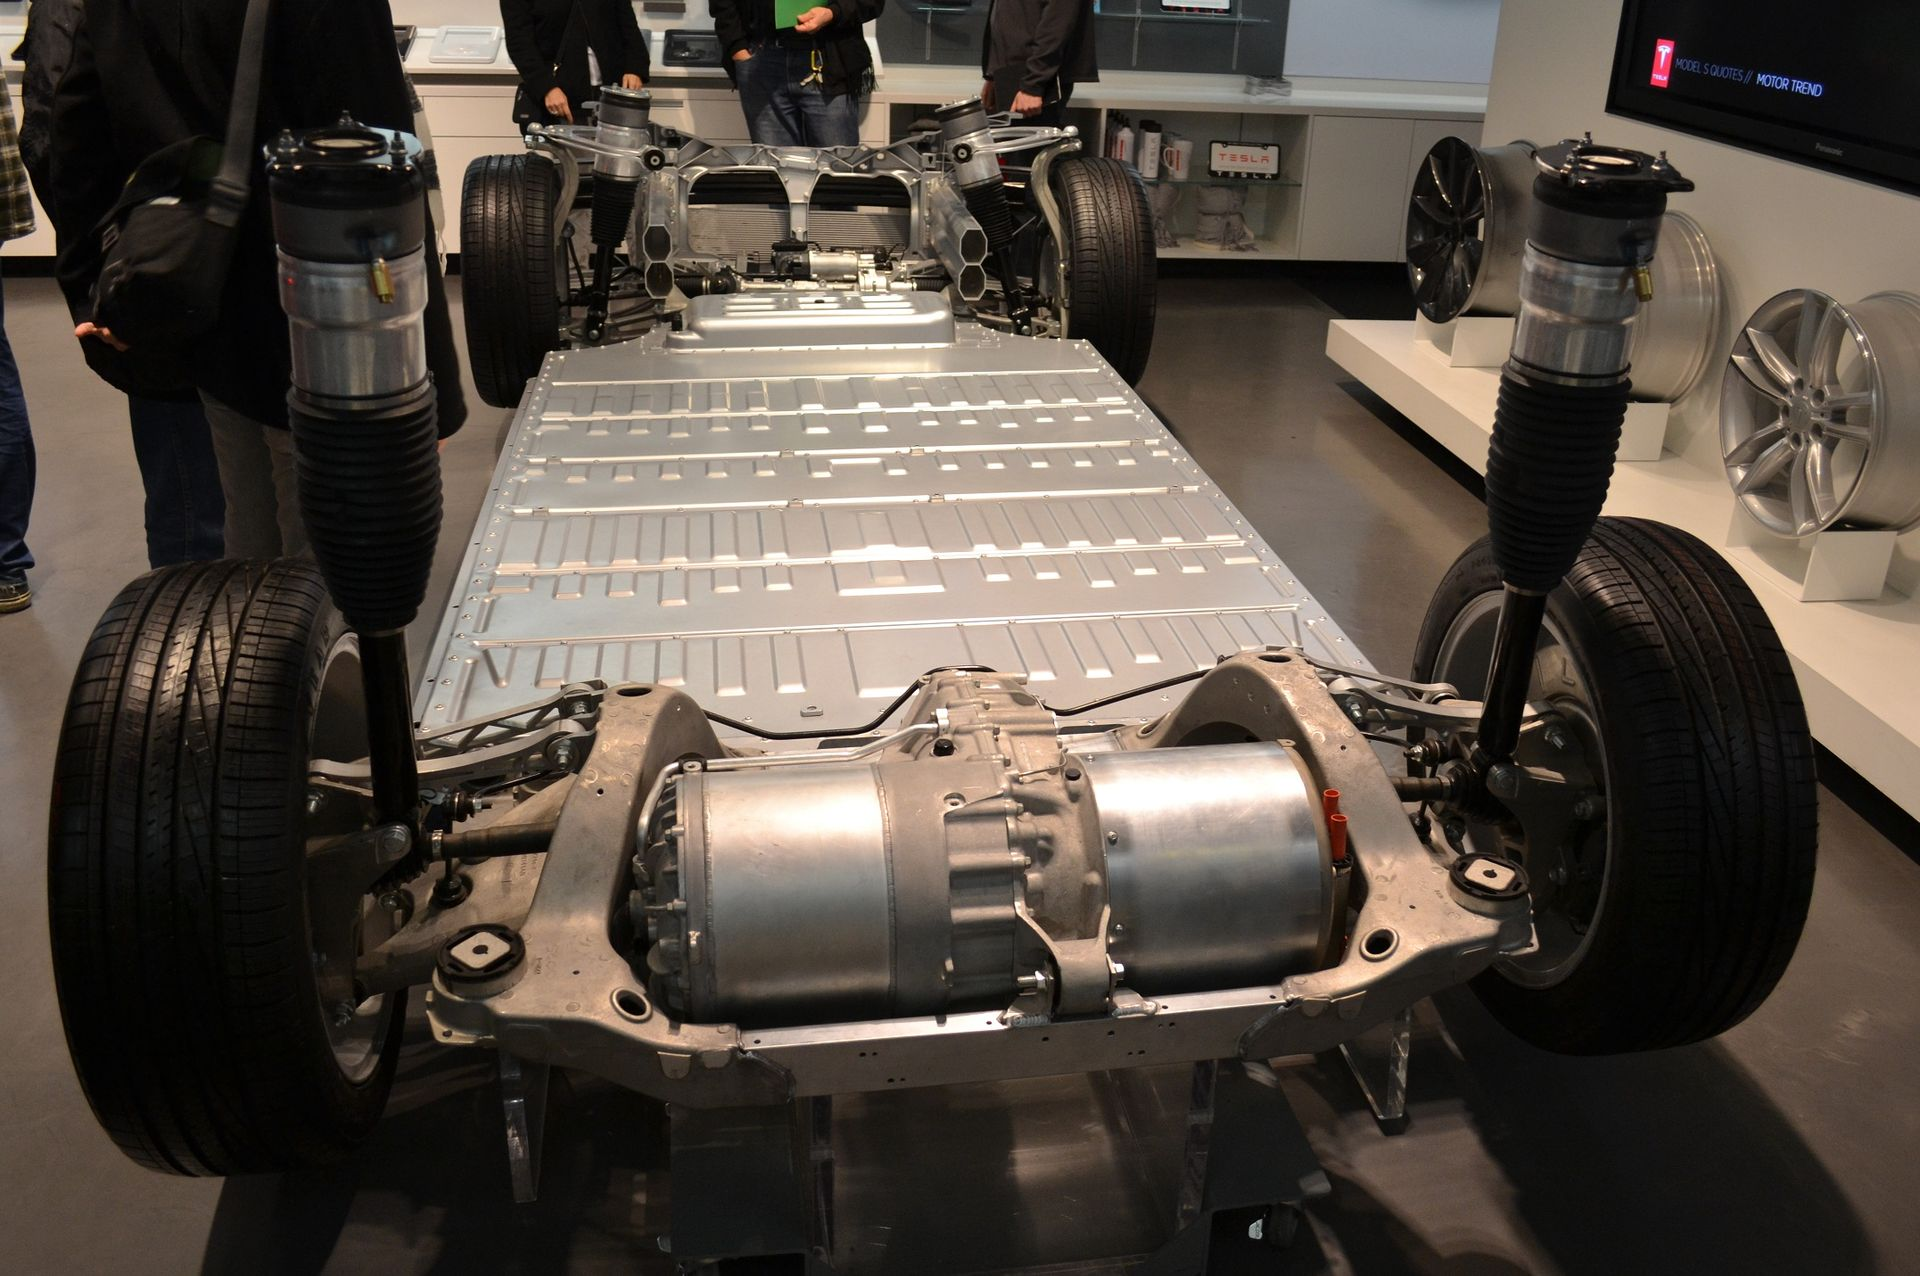
\includegraphics[width=0.99\textwidth]{./images/photos/tesla_car_electric_motor.jpg}\\
           Electric motor on Tesla Model S
     \end{center}
   }
  \end{column}
  \begin{column}{0.50\textwidth}
    \begin{itemize}
    {\small
      \item It exploits the interaction between an electric motor's magnetic field
            and current loops to generate force within the motor.
      \item It can be powered by
              \begin{itemize}
                  \item direct current (DC) sources (e.g. batteries), or
                  \item alternating current (AC) sources (e.g. the power grid).
             \end{itemize}
    }
    \end{itemize}
  \end{column}
\end{columns}

\end{frame}

%
%
%

\begin{frame}{The DC electric motor}

We will study a typical {\bf DC electric motor}.\\
\vspace{0.2cm}

\begin{columns}[t]
  \begin{column}{0.50\textwidth}
    \begin{center}
     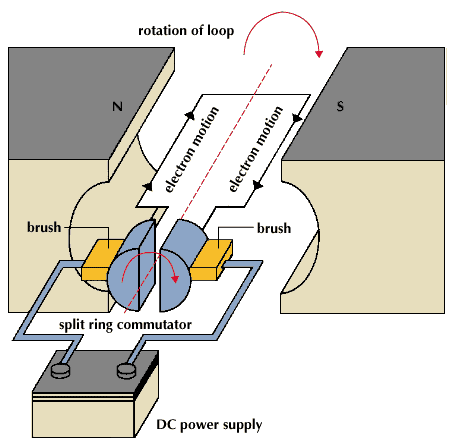
\includegraphics[width=0.99\textwidth]{./images/schematics/electric_motor_dc_01.png}\\
    \end{center}
  \end{column}
  \begin{column}{0.50\textwidth}
    {\small
    There are two main parts:
    \begin{itemize}
      \item The part which is stationary (called {\bf stator}) and includes the magnet.
      \item The part which rotates (called {\bf rotor}) -
                It turns a shaft to provide the mechanical power it generates (i.e. can be coupled to pulleys or gears and can do work).
    \end{itemize}
    }
    \begin{center}
        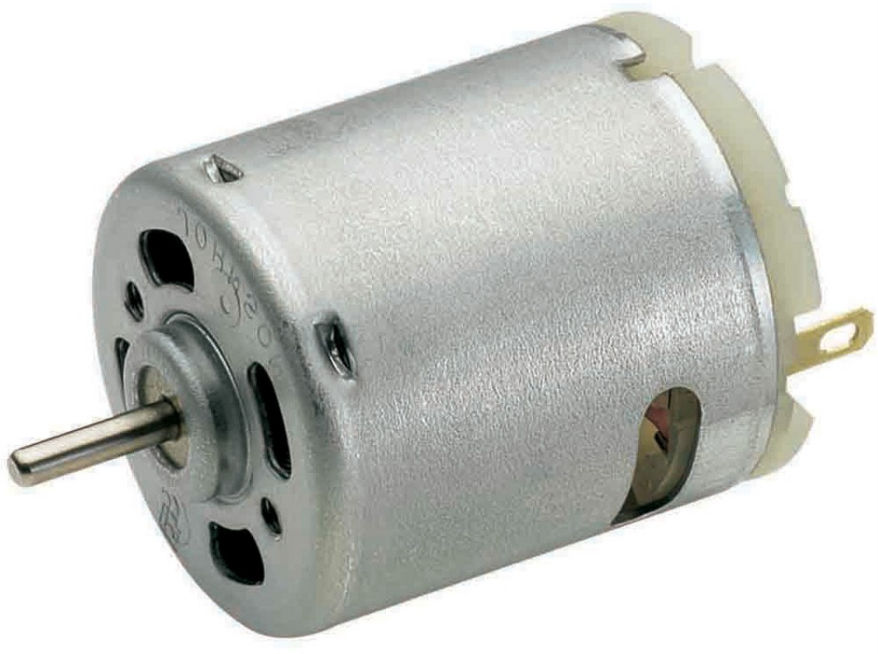
\includegraphics[width=0.50\textwidth]{./images/photos/electric_motor_dc_normal.jpg}\\
    \end{center}
  \end{column}
\end{columns}

\end{frame}

%
%
%

\begin{frame}{The DC electric motor}

\begin{columns}
  \begin{column}{0.50\textwidth}
    \begin{center}
     (a) Brushes are aligned with commutator segments.\\
     \vspace{0.3cm}
     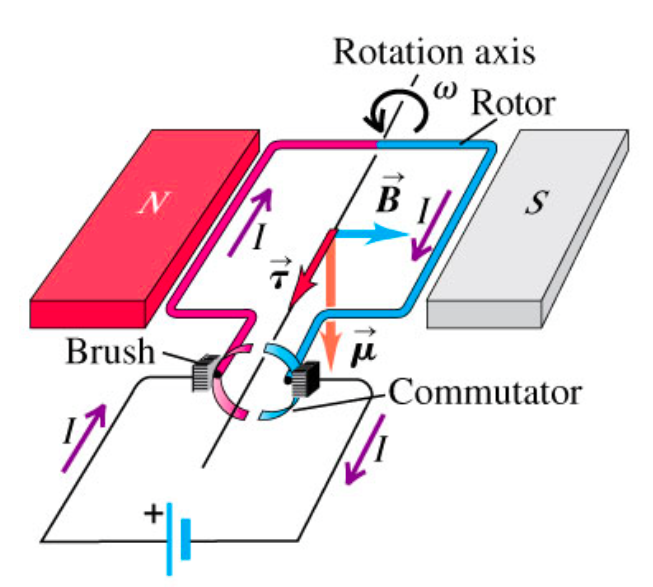
\includegraphics[width=0.99\textwidth]{./images/schematics/electric_motor_dc_operation_a.png}\\
    \end{center}
  \end{column}
  \begin{column}{0.50\textwidth}
    {\small
      \begin{itemize}
         \item Current flows into the red side of the rotor and out of the blue side.
         \item Magnetic forces:\\
          \begin{center}
              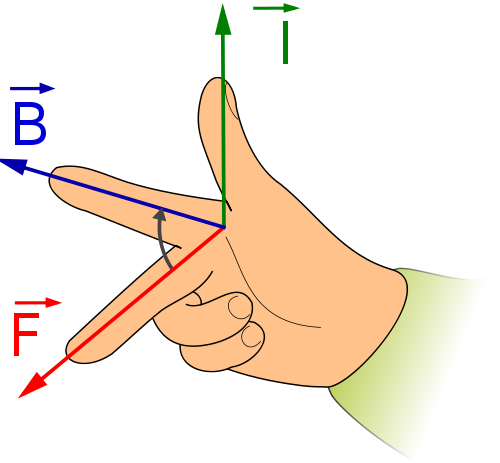
\includegraphics[width=0.45\textwidth]{./images/schematics/right_hand_rule_fbi.png}\\
           \end{center}
            \begin{itemize}
                \item on {\color{red}left-hand side}: downwards
                \item on {\color{blue}right-hand side}: upwards
            \end{itemize}
         \item The magnetic torque causes the rotor to {\bf spin counterclockwise}.
      \end{itemize}
    }
  \end{column}
\end{columns}

\end{frame}

%
%
%

\begin{frame}{The DC electric motor}

\begin{columns}
  \begin{column}{0.50\textwidth}
    \begin{center}
     (b) The rotor has turned 90$^{o}$.\\
     \vspace{0.3cm}
     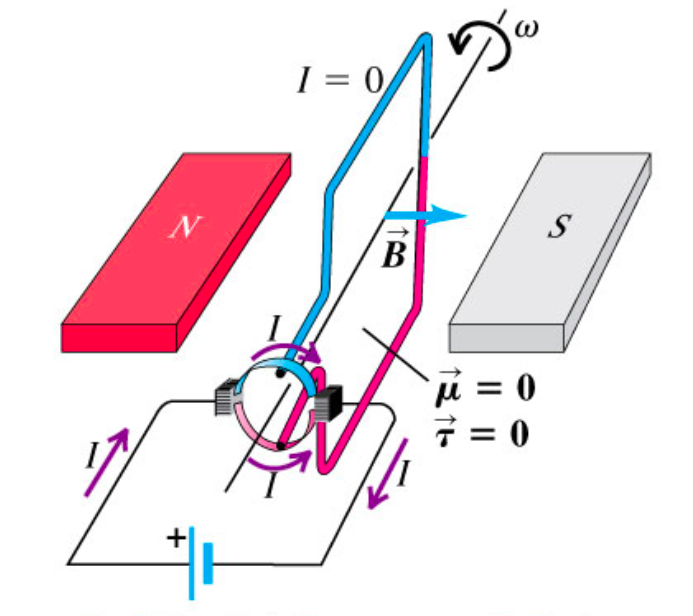
\includegraphics[width=0.99\textwidth]{./images/schematics/electric_motor_dc_operation_b.png}\\
    \end{center}
  \end{column}
  \begin{column}{0.50\textwidth}
  {\small
      \begin{itemize}
           \item Each brush is in contact with both commutator segments,
                     so the current bypasses the rotor altogether.
           \item {\bf No magnetic torque acts on the rotor}
      \end{itemize}
  }
  \end{column}
\end{columns}

\end{frame}

%
%
%

\begin{frame}{The DC electric motor}

\begin{columns}
  \begin{column}{0.50\textwidth}
    \begin{center}
     (c) The rotor has turned 180$^{o}$.\\
     \vspace{0.3cm}
     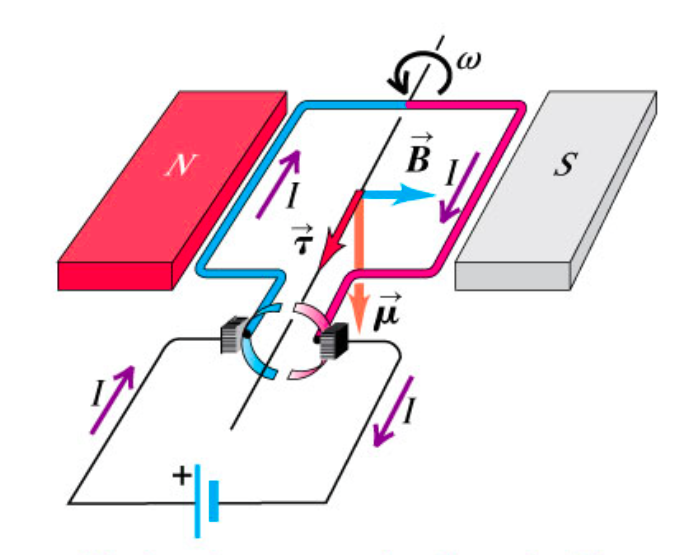
\includegraphics[width=0.99\textwidth]{./images/schematics/electric_motor_dc_operation_c.png}\\
    \end{center}
  \end{column}
  \begin{column}{0.50\textwidth}
  {\small
      \begin{itemize}
           \item The brushes are again aligned with commutator segments
                     This time the current flows into the blue side of the rotor and out of the red side.
         \item Magnetic forces:\\
            \begin{itemize}
                \item on {\color{blue}left-hand side}: downwards
                \item on {\color{red}right-hand side}: upwards
            \end{itemize}
           \item Therefore the magnetic torque again causes the rotor to {\bf spin counterclockwise}.
      \end{itemize}
  }
  \end{column}
\end{columns}

\vspace{0.2cm}

Question: What would happen if the current flow was unchanged
(e.g. always into the red side of the rotor and out of the blue side as in (a))?


\end{frame}

%
%
%

\begin{frame}{The DC electric motor and generators}

Note that the machine shown on the slide {\bf is either a motor, or a generator!}
There is a {\bf reciprocity between the two}.

\begin{columns}
  \begin{column}{0.70\textwidth}
    \begin{center}
     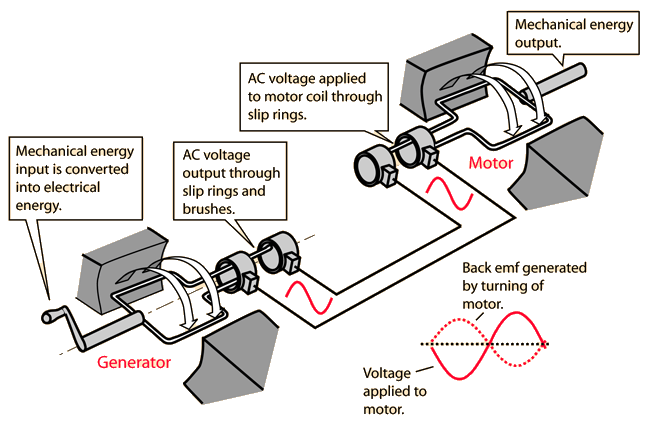
\includegraphics[width=0.99\textwidth]{./images/schematics/electric_motor_as_generator.png}\\
    \end{center}
  \end{column}
  \begin{column}{0.30\textwidth}
  {\scriptsize
    \begin{itemize}
     \item Examine what happens if, instead of putting a current through the loop to make it rotate, you rotate the loop manually.
     \item As loop rotates into a magnetic field, so there is an EMF in the circuit and current flows!
    \end{itemize}
  }
  \end{column}
\end{columns}

\end{frame}

%
%
%

\begin{frame}{The curl of the magnetic field}

Recall the {\bf circuital law} of electrostatics:
\begin{equation*}
    \vec{\nabla} \times \vec{E} = 0
\end{equation*}
It tells us that the {\bf electric field has no rotation} anywhere in space.\\
Hence, there are {\bf no closed field lines} in an electrostatic field.\\

\vspace{0.2cm}

\begin{columns}
  \begin{column}{0.50\textwidth}
    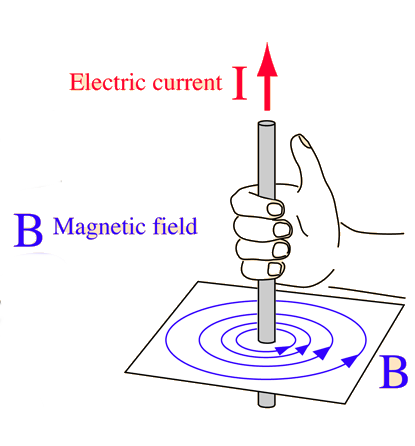
\includegraphics[width=0.75\textwidth]{./images/schematics/magnetic_field_around_wire_01.png}
  \end{column}
  \begin{column}{0.50\textwidth}
         {\bf How about the magnetic field?}\\
         \vspace{0.2cm}
         We have studied one example in detail (the magnetic field
         of an infinite straight wire) where we saw a very different
         behaviour:\\
         \vspace{0.2cm}
         The magnetic field lines {\bf loop back on themselves} (the magnetic
         field lines are always closed)!
  \end{column}
\end{columns}

\end{frame}

%
%
%

\begin{frame}{The curl of the magnetic field}

Magnetic field examples: The field lines {\bf loop back on themselves}!\\

\begin{center}
   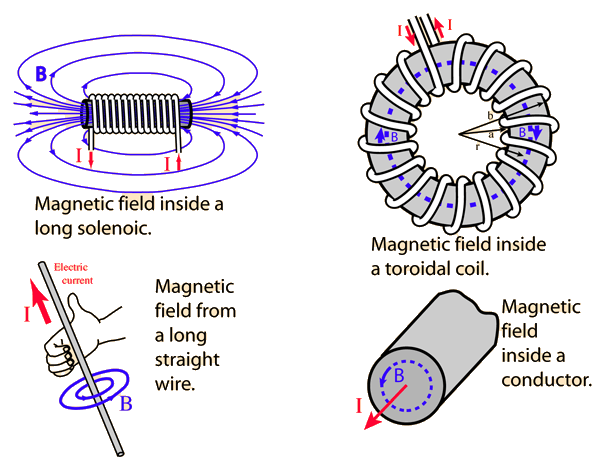
\includegraphics[width=0.77\textwidth]{./images/schematics/magnetic_field_examples.png}
\end{center}

\end{frame}

%
%
%

\begin{frame}{The curl of the magnetic field}

In the case of the infinitely-long straight conducting wire with current I,
we can easily calculate the line integral $\oint \vec{B}  d\vec{\ell}$  of the magnetic field
$\vec{B}$ along a closed circular trajectory.\\
\vspace{0.1cm}

\begin{columns}
  \begin{column}{0.30\textwidth}
    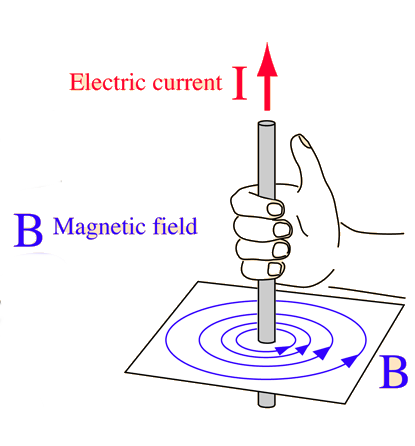
\includegraphics[width=0.77\textwidth]{./images/schematics/magnetic_field_around_wire_01.png}
  \end{column}
  \begin{column}{0.70\textwidth}
      As we have seen, $\vec{B}$ is given by:
      $\vec{B}(\vec{r}) = \frac{\mu_0I}{2\pi \rho} \hat{\phi}$
      whereas an infinitesimal step $d\vec{\ell}$ on a circular trajectory or radius $\rho$ is given by:
      $d\vec{\ell} = \rho \; d\phi \; \hat{\phi}$
  \end{column}
\end{columns}

\vspace{0.2cm}

Therefore:
\begin{equation*}
   \oint \vec{B} \cdot d\vec{\ell} =
      \oint \Big(  \frac{\mu_0I}{2\pi \rho} \hat{\phi} \Big) \cdot \Big( \rho d\phi \hat{\phi} \Big) =
      \frac{\mu_0I}{2\pi \cancel{\rho}} \cancel{\rho}  \oint \Big( \hat{\phi} \cdot \hat{\phi} \Big) d\phi =
      \frac{\mu_0I}{2\pi} \oint d\phi =
      \frac{\mu_0I}{\cancel{2\pi}} \cancel{2\pi} \Rightarrow
\end{equation*}

\begin{equation*}
   \oint \vec{B} \cdot d\vec{\ell} = \mu_0 I
\end{equation*}

\end{frame}

%
%
%

\begin{frame}{The curl of the magnetic field}

The previous result can be {\bf generalised for any closed path} around an infinite conductor.\\

\begin{columns}
  \begin{column}{0.20\textwidth}
    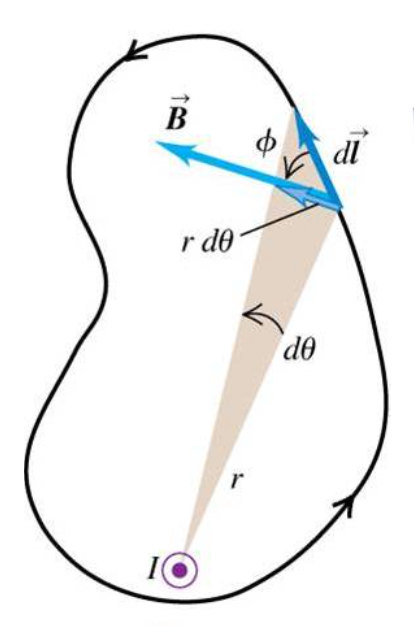
\includegraphics[width=0.90\textwidth]{./images/schematics/magnetic_field_path_integral_generalisation_any_shape.png}
  \end{column}
  \begin{column}{0.80\textwidth}
      \begin{equation*}
         \oint \vec{B} \cdot d\vec{\ell} = \oint |\vec{B}| |d\vec{\ell}| cos\phi \Rightarrow
         \oint \vec{B} \cdot d\vec{\ell} = \oint \Big( \frac{\mu_0 I}{2\pi \cancel{r}} \Big) \Big( \cancel{r} \; d\theta \Big) \Rightarrow
      \end{equation*}
      \begin{equation*}
         \oint \vec{B} \cdot d\vec{\ell} =  \frac{\mu_0 I}{2\pi} \oint d\theta =   \frac{\mu_0 I}{\cancel{2\pi}} \cancel{2\pi}  \Rightarrow
         \oint \vec{B} \cdot d\vec{\ell} =  \mu_0 I
      \end{equation*}
  \end{column}
\end{columns}

\vspace{0.2cm}

It can also be {\bf generalised for any number of conductors (currents)} passing through the loop.
In general:
\begin{equation*}
    \oint \vec{B} \cdot d\vec{\ell} = \mu_0 I_{encl}
\end{equation*}
where:
\begin{equation*}
     I_{encl} = \int_{S} \vec{j} \cdot d\vec{S}
\end{equation*}

\end{frame}

%
%
%

\begin{frame}{Ampere's law (integral form)}

\begin{columns}
  \begin{column}{0.22\textwidth}
    \begin{center}
     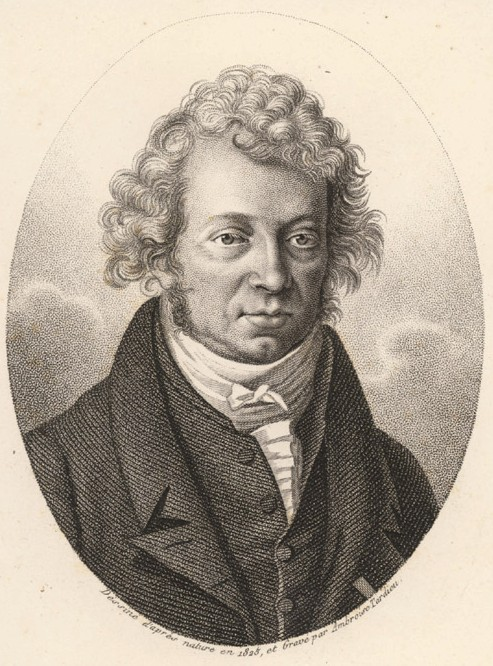
\includegraphics[width=0.70\textwidth]{./images/people/ampere.jpg}\\
     {\scriptsize
       Andr\'e Amp\`ere, 1775-1836\\
       French physicist and mathematician.\\
     }
    \end{center}
  \end{column}
  \begin{column}{0.78\textwidth}
     The general result we just saw is known as {\bf Ampere's law}:
     \begin{equation*}
        \oint_{L} \vec{B} \cdot d\vec{\ell} = \mu_0 I_{encl} = \mu_0 \int_{S} \vec{j} \cdot d\vec{S}
     \end{equation*}
     The line integral of the magnetic field $\vec{B}$ along a closed path L is proportional to the
     current passing though any surface S defined by L.
  \end{column}
\end{columns}

\vspace{0.2cm}
\noindent\rule{2cm}{0.4pt}\\
{\small
     We can draw some illuminating parallels with Gauss's law in electrostatics:
     \begin{equation*}
        \oint_{S} \vec{E} \cdot d\vec{S} = \frac{1}{\epsilon_0} Q_{encl} = \frac{1}{\epsilon_0} \int_{\tau} \rho d\tau
     \end{equation*}
     The surface integral of the electric field $\vec{E}$  through a closed surface S
     is proportional to the net charge contained in the volume $\tau$ defined by S.
}

\end{frame}

%
%
%

\begin{frame}{Ampere's law (differential form)}

Ampere's law in integral form is:
\begin{equation*}
    \oint_{L} \vec{B} \cdot d\vec{\ell} = \mu_0 I_{encl} = \mu_0 \int_{S} \vec{j} \cdot d\vec{S}
\end{equation*}

\begin{columns}
  \begin{column}{0.25\textwidth}
    \begin{center}
     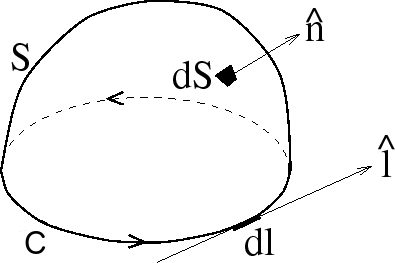
\includegraphics[width=0.99\textwidth]{./images/schematics/stokes_theorem_C.png}\\
    \end{center}
  \end{column}
  \begin{column}{0.75\textwidth}
     Stoke's theorem relates the line integral of a vector field with the surface integral
     of the curl of the field:
     \begin{equation*}
        \oint_{L} \vec{B} \cdot d\vec{\ell} = \int_{S} (\vec{\nabla} \times \vec{B}) \cdot d\vec{S}
     \end{equation*}
  \end{column}
\end{columns}

\vspace{0.3cm}

Applying Stoke's theorem Ampere's law becomes:
\begin{equation*}
    \int_{S} (\vec{\nabla} \times \vec{B}) \cdot d\vec{S} = \mu_0 \int_{S} \vec{j} \cdot d\vec{S} \Rightarrow
    \int_{S} \Big( \vec{\nabla} \times \vec{B} - \mu_0 \vec{j} \Big) \cdot d\vec{S} = 0
\end{equation*}
The above integral to be 0 for every surface S, hence:
\begin{equation*}
    \vec{\nabla} \times \vec{B} = \mu_0 \vec{j}
\end{equation*}

\end{frame}


%
%
%


\begin{frame}{Application of Ampere's Law: Field of toroidal coil}

Consider a toroidal (*) coil with N equally spaced circular windings carying current I.\\
\vspace{0.1cm}

\begin{center}
     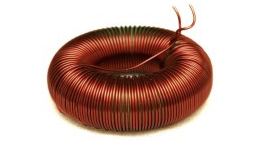
\includegraphics[width=0.53\textwidth]{./images/photos/toroidal_coil.png}
\end{center}

What is the {\bf magnetic field inside and outside the torus?}\\

\vspace{0.1cm}
\noindent\rule{2cm}{0.4pt}\\
{\small
   (*) A {\bf torus} is the surface generated by rotating a circle in 3-dimensional space about
       an axis that is coplanar with the circle (i.e. a doughnut shape)
}

\end{frame}



\begin{frame}{Application of Ampere's Law: Field of toroidal coil}

Inside the torus, the field is directed tangentially, as shown below, and it depends on the radius r.\\

\begin{columns}
  \begin{column}{0.33\textwidth}
    \begin{center}
     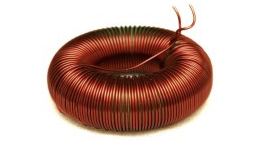
\includegraphics[width=0.95\textwidth]{./images/photos/toroidal_coil.png}\\
     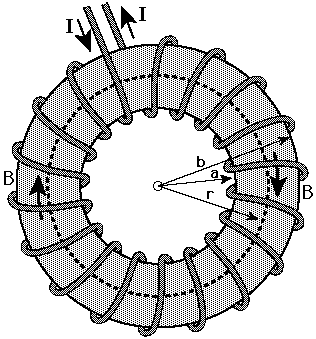
\includegraphics[width=0.95\textwidth]{./images/schematics/toroidal_coil_magnetic_field.png}\\
    \end{center}
  \end{column}
  \begin{column}{0.67\textwidth}
      Consider the path shown with a dashed line on the schematic:
      The magnitude of the magnetic field $|\vec{B}|$ is constant along the chosen path, and
      $\vec{B}$ is collinear with $ d\vec{\ell}$. Therefore:
     \begin{equation*}
        \oint_{L} \vec{B} \cdot d\vec{\ell} = |\vec{B}| 2\pi r
     \end{equation*}
     Since there are N windings, each carrying current I, the total current enclosed
     by the chosen path is:
     \begin{equation*}
        I_{encl} = N I
     \end{equation*}
  \end{column}
\end{columns}

\end{frame}

%
%
%

\begin{frame}{Application of Ampere's Law: Field of toroidal coil}

\begin{columns}
  \begin{column}{0.33\textwidth}
    \begin{center}
     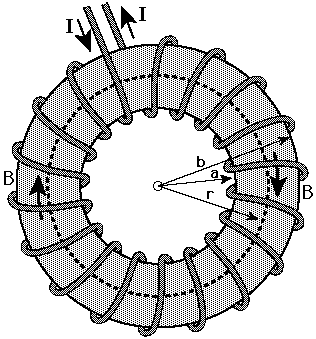
\includegraphics[width=0.90\textwidth]{./images/schematics/toroidal_coil_magnetic_field.png}\\
    \end{center}
  \end{column}
  \begin{column}{0.67\textwidth}
     Ampere's law in integral form is:
     \begin{equation*}
        \oint_{L} \vec{B} \cdot d\vec{\ell} = \mu_0 I_{encl}
     \end{equation*}
     So inside the torus:
     \begin{equation*}
         |\vec{B}| 2\pi r = \mu_0 N I \Rightarrow  |\vec{B}| = \frac{\mu_0 N I}{2\pi r}
     \end{equation*}

  \end{column}
\end{columns}

Hence the results of the magnetic field $\vec{B}$
can be summarised as follows:
    \begin{equation*}
      |\vec{B}| = \left\{ \begin{array}{l}
             0, \text{for $r < a$,} \\
             \frac{\mu_0 n I}{2\pi r}, \text{for $a < r < b$, and} \\
             0, \text{for $r > b$} \\
        \end{array} \right.
    \end{equation*}

\end{frame}


%
%

% starting reminder
{
\reminderslide

%
%
%

\begin{frame}{Calculus reminders}

You should try to prove both of these at home\\
\vspace{0.3cm}

{\bf BAC-CAB rule:}\\
\begin{equation*}
   \vec{\nabla} \cdot \Big( \vec{A} \times \vec{B} \Big) =
      \vec{B} \cdot \Big( \vec{\nabla} \times \vec{A} \Big) -
      \vec{A} \cdot \Big( \vec{\nabla} \times \vec{B} \Big)
\end{equation*}

\vspace{0.2cm}

{\bf The curl of $\vec{r}/|\vec{r}|^3$:}\\
\begin{equation*}
  \vec{\nabla} \times \frac{\vec{r}}{|\vec{r}|^3} =
      \left|
    \begin{array}{ccc}
      \hat{x} & \hat{y} & \hat{z} \\
      \frac{\partial}{\partial x} & \frac{\partial}{\partial y} & \frac{\partial}{\partial z} \\
      \frac{x}{\Big(x^2 + y^2 + z^2 \Big)^{3/2}} & \frac{y}{\Big(x^2 + y^2 + z^2 \Big)^{3/2}} & \frac{z}{\Big(x^2 + y^2 + z^2 \Big)^{3/2}}\\
    \end{array}
   \right| = 0
\end{equation*}

\begin{itemize}
  \item Recall that $\vec{r}/|\vec{r}|^3$ appears both in the Coulomb and Biot-Savart law.
\end{itemize}

\end{frame}

} % end reminder

%
%
%

\begin{frame}{Generalisation of the Biot-Savart law for a current density $\vec{j}$}

\begin{columns}
  \begin{column}{0.40\textwidth}
    \begin{center}
     \includegraphics[width=0.90\textwidth]{./images/schematics/biot_savart_current_density.png}\\
    \end{center}
  \end{column}
  \begin{column}{0.60\textwidth}

     At an earlier lecture, we studied the Biot-Savart law for a constant current I flowing over a linear path:
     \begin{equation*}
            \vec{B} = \frac{\mu_0I}{4\pi} \int_{L} \frac{d\vec{\ell} \times \vec{r}}{r^3}
     \end{equation*}
          where the line integral is over the elements $d\vec{\ell}$ along the conductor, and $\vec{r}$
          is the distance from $d\vec{\ell}$ to the point where we want to know the field.\\
      \vspace{0.2cm}
      The Biot-Savart law can be trivially generalised for an arbitrary current density $\vec{j}$:
    \begin{equation*}
        \vec{B} =
          \frac{\mu_0}{4\pi} \int_{\tau^{\prime}}
             \frac{\vec{j}(\pvec{r}') \times \vec{r}}{r^{3}} d\tau^{\prime}
    \end{equation*}
  \end{column}
\end{columns}


\end{frame}

%
%
%

\begin{frame}{The divergence and flux of the magnetic field}

Starting from the Biot-Savart law:
\begin{equation*}
        \vec{B} =
          \frac{\mu_0}{4\pi} \int_{\tau^{\prime}}
             \frac{\vec{j}(\pvec{r}') \times \vec{r}}{r^{3}} d\tau^{\prime}
\end{equation*}

we will calculate the divergence of $\vec{B}$.
The operator $\vec{\nabla}$ commutes with the integral and is applied to the integrant.
The BAC-CAB rules gives:
\begin{equation*}
         \vec{\nabla} \cdot \Big( \vec{j}(\pvec{r}') \times \frac{\vec{r}}{r^{3}} \Big) =
         \frac{\vec{r}}{r^{3}} \Big( \vec{\nabla} \times \vec{j}(\pvec{r}') \Big) -
         \vec{j}(\pvec{r}') \Big( \vec{\nabla} \times \frac{\vec{r}}{r^{3}} \Big)
\end{equation*}

The operator $\vec{\nabla}$ involves derivative of the unprimed variables
whereas the density $\vec{j}$ is a function of primed variables only, hence:
$\vec{\nabla} \times \vec{j}(\pvec{r}') = 0$.\\
\vspace{0.1cm}
As we have also seen:
$\vec{\nabla} \times \frac{\vec{r}}{r^{3}} = 0$.\\
\vspace{0.1cm}
Therefore:
\begin{equation*}
         \vec{\nabla} \cdot \vec{B} =  0
\end{equation*}

\end{frame}

%
%
%

\begin{frame}{The divergence and flux of the magnetic field}

The equation
\begin{equation*}
         \vec{\nabla} \cdot \vec{B} =  0
\end{equation*}
expresses the fact that {\bf there are no magnetic monopoles}.
Indeed, there is no point in space from where magnetic field lines {\em emanate from},
and they always loop back on themselves.\\

\vspace{0.2cm}
For the same reason, we expect that the magnetic flux through a closed surface is zero:
The field lines that from a closed surface eventually re-enter as they loop back on themselves.\\

Gauss' theorem tells us that:
\begin{equation*}
         \oint_{S} \vec{B} \cdot d\vec{S} = \int_{\tau} \vec{\nabla} \cdot \vec{B} d\tau
\end{equation*}

But $\vec{\nabla} \cdot \vec{B} =  0$, hence:
\begin{equation*}
         \oint_{S} \vec{B} \cdot d\vec{S} = 0
\end{equation*}

\end{frame}

%
%
%

\begin{frame}{The vector potential}

Recall that, in electrostatics, the circuital law:
\begin{equation*}
      \vec{\nabla} \times \vec{E} = 0
\end{equation*}
allowed us to write the electric field $\vec{E}$ as the gradient of a scalar field
(recall that $\vec{\nabla} \times \Big( \vec{\nabla} \phi \Big) =0$
for {\em any} scalar function $\phi$).
That scalar field was the potential V:
\begin{equation*}
      \vec{E} = - \vec{\nabla} V
\end{equation*}
By substituting the above into Gauss's law,
we found that the scalar potential V satisfies the so-called {\em Poisson} equation:
\begin{equation*}
      \vec{\nabla}^{2} V = - \frac{\rho}{\epsilon_0}
\end{equation*}

\noindent\rule{2cm}{0.4pt}\\
{\scriptsize
This single 2$^{nd}$ order p.d.e for the electric potential V, is equivalent with the following coupled system of
two 1$^{st}$ order p.d.e's: $\vec{\nabla} \times \vec{E} = 0$ and  $\vec{\nabla} \cdot \vec{E} = \rho/\epsilon_0$.
Using the appropriate boundary conditions we can solve the Poisson's
equation to determine V and, thus, determine $\vec{E}$.\\
}

\end{frame}

%
%
%

\begin{frame}{The vector potential}

Similarly, the relation
\begin{equation*}
      \vec{\nabla} \cdot \vec{B} = 0
\end{equation*}
allows us to express the magnetic field $\vec{B}$ as the rotation of a
vector field (recall that $\vec{\nabla} \cdot \Big( \vec{\nabla} \times \vec{A} \Big) =0$
for {\em any} vector field $\vec{A}$):

\begin{equation*}
      \vec{B} = \vec{\nabla} \times \vec{A}
\end{equation*}
We call $\vec{A}$ the {\bf vector potential}.

\vspace{0.2cm}

Substituting the above definition into Ampere's law:
\begin{equation*}
     \vec{\nabla} \times \vec{B} = \mu_{0} \vec{j} \Rightarrow
     \vec{\nabla} \times \Big( \vec{\nabla} \times \vec{A}  \Big) =  \mu_{0} \vec{j} \Rightarrow
\end{equation*}
\begin{equation*}
     \vec{\nabla} \Big( \vec{\nabla} \cdot \vec{A}  \Big) - \vec{\nabla}^2 \vec{A}   =  \mu_{0} \vec{j}
\end{equation*}

\end{frame}

%
%
%

\begin{frame}{The vector potential}

One can add to V {\em any function} $\lambda$ whose gradient is zero ($\vec{\nabla} \lambda = 0$):
\begin{equation*}
   V \rightarrow V^{\prime} = V + \lambda
\end{equation*}
and the {\bf physics would remain unchanged}!\\
\vspace{0.1cm}

Similarly, we can add to $\vec{A}$  {\em any function} $\vec{\Lambda}$
whose curl vanishes ($\vec{\nabla} \times \vec{\Lambda} = 0$):
\begin{equation*}
   \vec{A} \rightarrow \pvec{A}' = \vec{A} + \vec{\Lambda}
\end{equation*}
and the {\bf physics would remain unchanged}!\\
\vspace{0.1cm}

We can use this freedom to eliminate the divergence of $\vec{A}$ ($\vec{\nabla} \vec{A} = 0$).
With this condition, $\vec{A}$ satisfies the following p.d.e.:
\begin{equation*}
   \vec{\nabla}^2 \vec{A}   =  - \mu_{0} \vec{j}
\end{equation*}

This expression is very similar to our known {\em Poisson} equation.
In fact, it is nothing more than a {\em vector of Poisson} equations.

\end{frame}

%
%
%

\begin{frame}{Maxwell's equation we know so far}

In vacuum (static case):

\begin{center}
 {
  \begin{table}[H]
    \begin{tabular}{|l|c|c|}
      \hline
          & {\it Integral form} & {\it Differential form} \\
      \hline
      {\bf Gauss's law} &
        $\oint \vec{E} \cdot d\vec{S} = Q_{enclosed} / \epsilon_0$ &
        $\vec{\nabla} \cdot \vec{E} = \rho / \epsilon_0$ \\

      {\bf Circuital law} &
        $\oint \vec{E} \cdot d\vec{\ell} = 0$ &
        $\vec{\nabla} \times \vec{E} = 0$ \\

      {\bf Gauss's law} (magn.) &
        $\oint \vec{B} \cdot d\vec{S} = 0$ &
        $\vec{\nabla} \cdot \vec{B} = 0$ \\

      {\bf Ampere's law} &
        $\oint \vec{B} \cdot d\vec{\ell} = \mu_{0} I $ &
        $\vec{\nabla} \times \vec{B} = \mu_{0} \vec{j}$ \\

      \hline
    \end{tabular}
  \end{table}
 }
\end{center}

\end{frame}

% ------------------------------------------------------------------------------
% ------------------------------------------------------------------------------

%
% What to remember
%

\renewcommand{\lecturesummarytitle}{Main points to remember }

\renewcommand{\summarizedlecture}{6 }


\begin{frame}{Lecture \summarizedlecture - \lecturesummarytitle}

\begin{itemize}

\item
  At distance $\rho$, the force between two parallel straight
  conductors of length L carrying current $I_1$ and $I_2$,
  respectively, is:
  \begin{equation*}
    F = \frac{\mu_0 I_{1} I_{2} L}{2\pi \rho}
  \end{equation*}
  The force is attractive if both currents flow in the same direction, and
  repulsive if the two currents flow in opposite directions.

\item
  One Ampere is the amount of current that,
  if maintained between those conductors produces a force of 2
  $\times$ $10^{-7}$ N per metre of length.

\item
  The magnetic dipole moment $\vec{m}$ of a current loop is defined as
  \begin{equation*}
      \vec{m} = I \vec{S}
   \end{equation*}

\item
  The magnetic moment $\vec{T}$ of a magnet is a quantity that
  determines the torque it will experience in an external magnetic field.
  \begin{equation*}
      \vec{T} = \vec{m} \times \vec{B}
  \end{equation*}

\end{itemize}

\end{frame}

%
%
%

\begin{frame}{Lecture \summarizedlecture - \lecturesummarytitle (cont'd)}

\begin{itemize}

\item
    {\bf Ampere's law} in integral form:
     \begin{equation*}
        \oint_{L} \vec{B} \cdot d\vec{\ell} = \mu_0 I_{encl} = \mu_0 \int_{S} \vec{j} \cdot d\vec{S}
     \end{equation*}
     The line integral of the magnetic field $\vec{B}$ along a closed path L is proportional to the
     current passing though any surface S defined by L.

\vspace{0.2cm}

\item
    {\bf Ampere's law} in differential form:
    \begin{equation*}
       \vec{\nabla} \times \vec{B} = \mu_0 \vec{j}
    \end{equation*}
    The curl $\vec{B}$ is proportional to the local current density $\vec{j}$.

\vspace{0.2cm}

\item
    The magnetic field inside a toroidal coil with n windings, each carrying current I, is:
     \begin{equation*}
          |\vec{B}| = \frac{\mu_0 n I}{2\pi r}
     \end{equation*}
     where r is the distance from the centre of the coil.

\end{itemize}

\end{frame}

%
%
%

\begin{frame}{Lecture \summarizedlecture - \lecturesummarytitle (cont'd)}

\begin{itemize}

\item
      The relation:
      \begin{equation*}
              \vec{\nabla} \cdot \vec{B} = 0
      \end{equation*}
      allows us to express $\vec{B}$ as the curl of a vector field  $\vec{A}$:
      \begin{equation*}
             \vec{B} = \vec{\nabla} \times \vec{A}
      \end{equation*}
      We call $\vec{A}$ the {\bf vector potential}.

\item
     There is some freedom in determining $\vec{A}$:
    \begin{itemize}
         \item Adding to it a function whose curl is zero leaves the physics unchanged.
         \item We use this freedom to eliminate the divergence of $\vec{A}$ ($\vec{\nabla} \cdot \vec{A} = 0$).
    \end{itemize}

\item
     The vector potential $\vec{A}$ satisfies the following equation:
     \begin{equation*}
         \vec{\nabla}^2 \vec{A}   =  - \mu_{0} \vec{j}
     \end{equation*}
     (each component of $\vec{A}$ satisfies a Poisson equation).

\end{itemize}

\end{frame}


%
% Plan for the next lecture
%

\begin{frame}{At the next lecture (Lecture \nextlecture)}

In the next lecture, we will study the magnetic properties of materials:
\vspace{0.2cm}
\begin{itemize}
  \item diamagnetism
  \item paramagnetism
  \item ferromagnetism
\end{itemize}

\end{frame}

% ------------------------------------------------------------------------------
% ------------------------------------------------------------------------------
